\documentclass[a4paper]{article}
%\usepackage[top=30pt,left=30pt,right=30pt]{geometry}
\usepackage[german,english]{babel}
%\usepackage[utf8]{inputenc}
\usepackage{amsmath}
\usepackage{amssymb}
\usepackage{amsthm}
\usepackage{graphicx}
\usepackage{caption}
\usepackage{fontspec}
\usepackage{mdframed}
\usepackage{pxfonts}
\usepackage{wasysym}
\usepackage{framed}
\usepackage{xcolor}
\usepackage{makeidx}
\usepackage{csquotes}
\usepackage[pdfborder={0 0 0}]{hyperref}
\usepackage{stmaryrd}
\usepackage{titlesec}
\titleformat{\paragraph}{\normalfont\itshape}{}{}{}

\newcounter{lecref}[section]
\numberwithin{lecref}{section}
%\setcounter{lecref}{4}
\setcounter{section}{-1}

\newtheorem{theorem}[lecref]{Theorem}
\newtheorem*{Theorem}{Theorem}
\newtheorem{example}[lecref]{Example}
\newtheorem*{Example}{Example}
\newtheorem{definition}[lecref]{Definition}
\newtheorem*{Definition}{Definition}
\newtheorem{lemma}[lecref]{Lemma}
\newtheorem*{Lemma}{Lemma}
\newtheorem{claim}[lecref]{Claim}
\newtheorem*{Claim}{Claim}
\newtheorem{remark}[lecref]{Remark}
\newtheorem*{Remark}{Remark}
\newtheorem{algorithm}[lecref]{Algorithm}
\newtheorem*{Algorithm}{Algorithm}
\newtheorem{corollary}[lecref]{Corollary}
\newtheorem*{Corollary}{Corollary}
\newtheorem{proposition}[lecref]{Proposition}
\newtheorem*{Proposition}{Proposition}
\newtheorem{revision}[lecref]{Revision}
\newtheorem*{Revision}{Revision}

\def\ifempty#1{\def\temp{#1} \ifx\temp\empty }

% useful control sequences for mathematical notation
\newcommand{\Abs}[1]{\left|#1\right|}
\newcommand{\Set}[1]{\left\{#1\right\}}
\newcommand{\SetDef}[2]{\left\{#1\,\mid\,#2\right\}}
\newcommand{\IP}[2]{\left\langle#1, #2\right\rangle}
\newcommand{\Norm}[1]{\left\|{\ifempty{#1}\cdot\else#1\fi}\right\|}
\newcommand{\Max}[1]{\max{\Set{#1}}}
\newcommand{\Min}[1]{\min{\Set{#1}}}
\newcommand{\Sup}[1]{\sup{\Set{#1}}}
\newcommand{\Powerset}[1]{{\mathbb P}(#1)}
\newcommand{\IntRange}[2]{#1, \dots\ifempty{#2}\else, #2\fi}

\def\vec2#1#2{\begin{pmatrix} #1 \\ #2 \end{pmatrix}}
\def\vec3#1#2#3{\begin{pmatrix} #1 \\ #2 \\ #3 \end{pmatrix}}
\newcommand{\noproof}[1]{A proof for Theorem~\ref{#1} is not provided.}
\newcommand{\dotted}[1]{\:\dot{#1}\:}  % dot has too little margin

% German translation
\newcommand{\dt}[1]{(dt. \enquote{\foreignlanguage{german}{#1}})}

% essential control sequences
%% \xRightarrow: \xrightarrow for \rightarrow like \xRightarrow for \Rightarrow
\makeatletter
\newcommand{\xRightarrow}[2][]{\ext@arrow 0359\Rightarrowfill@{#1}{#2}}
\makeatother

% double \tilde
\newcommand{\ttilde}[1]{\tilde{\raisebox{0pt}[0.85\height]{$\tilde{#1}$}}}

% typesetting settings
\parindent0pt
\setlength{\parskip}{.6em}
\setmainfont{CMU Serif}

% TODO: span?
\DeclareMathOperator{\rank}{rank}
\DeclareMathOperator{\diag}{diag}
\DeclareMathOperator{\detm}{det}
\DeclareMathOperator{\perm}{perm}
\DeclareMathOperator{\sign}{sign}
\DeclareMathOperator{\degree}{deg}
\DeclareMathOperator{\im}{image}
\DeclareMathOperator{\ke}{kernel}
\DeclareMathOperator{\spec}{spec}
\DeclareMathOperator{\prop}{probability}
\DeclareMathOperator{\Hom}{Hom}
\DeclareMathOperator{\argmax}{argmax}
\DeclareMathOperator{\argmin}{argmin}
\DeclareMathOperator{\vol}{vol}  % volume
\DeclareMathOperator*{\bigtimes}{\vartimes}
\DeclareMathOperator{\dom}{dom}





\newcommand{\dateref}[1]{%
  \begin{mdframed}[backgroundcolor=gray!10,innerbottommargin=0pt,innertopmargin=0pt]
    \paragraph{\textit{$\downarrow$ This lecture took place on #1.}}%
  \end{mdframed}%
}

% metadata
\title{
  Introduction to Functional Analysis \\
  \large{Lecture notes, University of Technology, Graz} \\
  based on the lecture by Martin Holler
}
\date{\today}
\author{Lukas Prokop}

\makeindex
\begin{document}

\maketitle
\tableofcontents

\section{Introduction}

\dateref{2019/03/05}

\begin{itemize}
	\item Function Analysis, mostly Linear Functional Analysis
	\item Goal: Transfer objects and results for linear algebra and analysis to infinite-dimensional function spaces
	\item e.g. $\mathbb R^n, \mathbb C^n \mapsto$ vector spaces $U, V$ \\
		matrices $A \in \mathcal M^{n \times m} \mapsto$ operators $A \in \mathcal L(U, V)$ \\
		functions $f: \mathbb R^n \to \mathbb R \mapsto$ functionals $f: U \to \mathbb R$
	\item Furthermore we discuss inner products, orthogonality, connectedness, eigenvalues
	\item Fields of application
	  \begin{itemize}
	  	\item basis of Applied Mathematics
	  	\item partial differential equations
	  	\item physical modelling
	  	\item inverse problems (operator $A$ models some physical measurement process)
	  	\item Optimization and optimal control
	  \end{itemize}
\end{itemize}

A motivating example was presented with slides.

\subsection{Application examples}

Let $K: U \to \mathbb R^m$ with $U$ as vector space describe a physical model.
For example, $K$ is a Fourier/Radon/X-ray transform (MR/CT/PET imaging) or
$K u = y(1)$ where $y: [0, 1] \to \mathbb R^m$ solves $y'(t) = y(t) + u(t)$ and $y(0) = 0$.

\index{Inverse problems}
Another example is the class of so-called \emph{inverse problems}.
Given $d = ku$, find $u$.
Typically inversion of $K$ is ill-constrained. Solution is typically non-unique.

Approach: Solve $\min_{u \in U} \lambda \Norm{Ku - d}_2 + \Norm{u}_k$ where $\Norm{z}_2 \coloneqq \sqrt{\sum_{i=1}^n z_i^2}$ and $\Norm{\cdot}_u$ is a norm on $U$.
Or alternatively, let $U = \mathcal C^1([0,1]^2)$ and solve $\min_{u \in U} \lambda \Norm{ku - d}_2 + \sqrt{\int_{[0,1]^2} \Abs{\nabla u(x)}^2 \, dx}$.

Other examples are JPEG compression and upsampling of images.

\subsection{Our first problem}

Let $U \coloneqq \mathcal C^1([0,1]^2)$ be a normed space, $K: U \to \mathbb R^m$ linear.
Solve $\min_{u \in U} \lambda \Norm{Ku - d} + \sqrt{\int_{[0,1]^2} \Abs{\nabla u(x)}^2 \, dx}$.
The question is: does such a solution exist?

We have a background in finite-dimensional vector spaces.
We consider a special case to apply the theories we already know.

So we consider a discrete setting. Let $U: \mathbb R^n$ and $\nabla: \mathbb R^n \to \mathbb R^k$ is a discrete gradient.
In 1D, we have $u = (u_i)_{i} \in \mathbb R^m$ and $u_i = u(x_i) \implies u' \approx u(x_{i+1}) - u(x_i) = u_{i+1} - u_i$.
Consider $\min_{u \in \mathbb R^n} \Norm{\nabla u}_2 + \lambda \Norm{Ku - d}_2$ as problem.

Does there exist a solution to this problem assuming $\lambda > 0$, $K: \mathbb R^n \to \mathbb R^m$ linear and $\nabla: \mathbb R^n \to \mathbb R^k$ linear.

\begin{proof}
  \begin{description}
  	\item[Case 1 (trivial model):]
  	  Let $m = n$. $K_n = u$
  	  \begin{align} \min_{u \in \mathbb R^n} \Norm{\nabla u}_2 + \lambda \Norm{u - d}_2 \label{p1} \end{align}
  	  Take $(u_n)_{n \in \mathbb N}$ in $\mathbb R^n$ such that $\lim _{n \to \infty} \Norm{\nabla u_1}_2 +  \lambda \Norm{u_n - d}_2 = \inf_{u \in \mathbb R} \Norm{\nabla u}_2 + \lambda \Norm{u - d}_2$.
  	  It holds that $C = \lambda \Norm{d}_2 \geq \inf_{u \in \mathbb R} \Norm{\nabla u}_2 + \lambda \Norm{d}_2$.
  	  Without loss of generality, we can assume that $2C \geq \Norm{\nabla u_n}_2 + \lambda \Norm{u_n - d}_2 \forall n \in \mathbb N$
  	  \[ \implies \lambda \Norm{u_1}_2 \leq \lambda \Norm{u_n - d}_2 + \lambda \Norm{d}_2 \leq \Norm{\nabla u_k}_2 + \lambda \Norm{u_n - d}_2 - \lambda \Norm{d}_2 \leq 2C + \lambda \Norm{d}_2  \]
  	  $(\Norm{u_n}_2)_n$ is bounded. So the Bolzano-Weierstrass theorem applies and $(u_n)_{n \in \mathbb N}$ admits a convergent subsequence $(u_{n_i})_{i \in \mathbb N}$.
  	  Take $u \in \mathbb R^n$. $u_{n_i} \to u$ as $i \to \infty$.

  	  Now: Show that $u$ solves Problem~\eqref{p1}. $\nabla$ is continuous. $\Norm{\cdot}_2$ is continuous.
  	  \[ \inf_{u \in U} \Norm{\nabla u}_2 + \lambda \Norm{u - d}_2 = \lim_{i \to \infty} \Norm{\nabla u_{n_i}} + \lambda \Norm{u_{n_i} - d}_2 = \Norm{\nabla \hat{u}}_2 + \lambda \Norm{\hat{u} - d}_2 \]
  	  This implies that $\hat u$ is the solution to the problem of this first case.

  	  Ingredients of this proof where:
  	  \begin{itemize}
  	  	\item boundedness
  	  	\item compactness
  	  	\item continuity of $\nabla$, $\Norm{\cdot}_2$
  	  \end{itemize}
  	\item[Case 2 ($K$ arbitrary):]
  	  \begin{enumerate}
  	  	\item
	  	  $K$ arbitrary does not provide boundedness anymore.
	  	  Define $X \coloneqq \ke(\nabla) \cap \ke(k)$ and
	  	  \[ X^\bot \coloneqq \SetDef{x \in \mathbb R^n}{(x, y) \coloneqq \sum_{i=1}^n x_i y_i = 0 \forall y \in X} \]
	  	  Then we apply results from linear algebra:
	  	  \[ \mathbb R^n: X \oplus X^\bot \qquad \text{ i.e. } \forall u \in \mathbb R^n: \exists! u_1 \in X, u_2 \in X^\bot: u = u_1 + u_2 \]
	  	  \index{Orthogonal complement}
	  	  Recall, that $X^\bot$ is called \emph{orthogonal complement}.

	  	  \begin{claim}
	  	    If $\hat u$ solves $\min_{u \in X^\bot} \Norm{\nabla u}_2 + \lambda \Norm{Ku - d}_2$. Then $\hat{u}$ solves Problem~\eqref{p1}.
	  	  \end{claim}
	  	  \begin{proof}
	  	  	Let $\hat u$ be a solution on $X^\bot$.
	  	  	Take $u \in \mathbb R^n$ arbitrary. We write $u = u_1 + u_2 \in X \times X^\bot$. Now we have:
	  	  	\begin{align*}
	  	  	  \Norm{\nabla u}_2 + \lambda \Norm{ku - d}_2
	  	  	  	&= \Norm{\nabla (u_1 + u_2)}_2 + \lambda \Norm{k (u_1 + u_2) - d}_2 \\
	  	  	  	&= \Norm{\nabla u_2}_2 + \lambda \Norm{ku_2 - d}_2 \\
	  	  	  	&\geq \Norm{\nabla \hat u}_2 + \lambda \Norm{K\hat u - d}_2
	  	  	\end{align*}
	  	  	Thus $\hat u$ solves our problem~\eqref{p1}.
	  	  \end{proof}

	  	  Take again $(u_n)_{n \in \mathbb N}$ be such that $u_n \in X^\bot \forall n$ and
	  	  \[ \lim_{n \to \infty} \Norm{\nabla u_n}_2 + \lambda \Norm{k u_n - d}_2 = \inf_{u \in X^\bot} \Norm{\nabla_u}_2 + \lambda \Norm{ku - d}_2 \]
	  	  Write $u_1 = u_n^1 + u_n^2 \in \ke(\nabla) + \ke(\nabla)^\bot$.
	  	  $\nabla: \ke(\nabla)^\bot \to \im(\nabla)$ is bijective.
	  	  Since $\nabla v = 0$ for $v \in \ke(\nabla)^\bot \implies v \in \ke(\nabla) \implies \Norm{v_2} = (v, v) = 0$.
	  	  Thus, $\nabla^{-1}: \im(\nabla) \to \ke(\nabla)^\bot$ exists and is continuous.
	  	  \begin{align*}
	  	  	\implies \Norm{u_n^2}_2 &= \Norm{\nabla^{-1} \nabla u_n^2}_2 = \Norm{\nabla^{-1}} \cdot \Norm{\nabla u_n^2}_2 \leq \Norm{\nabla^{-1}} \\
	  	  		&\leq \Norm{\nabla^{-1}} \left(\Norm{\nabla u_n^2}_2 + \lambda \Norm{K u_n - d}_2\right) \\
	  	  		&= \Norm{\nabla^{-1}} \left(\underbrace{\Norm{\nabla u_n}_2}_{= \Norm{\nabla u_n}_2} + \lambda \Norm{K u_n - d}_2\right) \\
	  	  		&< C \text{ for some } C > 0
	  	  \end{align*}
	  	  Than $\Norm{u_n^2}_2$ bounded.
	  	\item Show $(u_n^1)_n$ is bounded. $K: X^\bot \cap \ker(\nabla) \to \im(K)$ is bijective.
	      Since $Kv = 0$ for $v \in X^\bot \cap \ke(\nabla) \implies v \in \ke(K)$. Hence $v \in \ke(K) \cap \ke(\nabla) = X \implies v \in X \cap X^\bot \implies v = 0$.
	      Hence $K^{-1}: \im(K) \to X^\bot \cap \ke(\nabla)$ exists and is continuous.
	      \begin{align*}
	      	\implies \Norm{u_n^n}_2 &= \Norm{K^{-1} K u_n^n}_2 \leq \Norm{K^{-1}} \Norm{K u_{n}^n}_2 \\
	      		&= \frac{\Norm{K}}{\lambda} \left(\lambda \Norm{K (u_1^n + u_2^n) - K u_n^n}_2 + \Norm{\nabla u_n}_2\right) \\
	      		&\leq \frac{\Norm{K}}{\lambda} \left(\underbrace{\lambda \Norm{K u_1 - d}_2}_{\text{bounded}} + \underbrace{\Norm{\nabla u_n}_2 + \lambda \Norm{d - K u_1^2}}_{\text{bounded because $u_n^2$ is bounded}}\right) \\
	      		&< D \text{ for some } D > 0 \\
	      	\implies (u_n^n)_n \text{bounded} &\implies (u_n) = (u_n^n + u_n^n)_n \text{ is bounded}
	      \end{align*}
	      $\implies (u_n)_n$ admits a subsequence converging to some $\hat u$.
	      As in Case 1, $\hat u$ is a solution to Problem~\eqref{p1}.
	  \end{enumerate}
  \end{description}
  In summary,
  \begin{enumerate}
  	\item $\min_{u \in U} \lambda \Norm{Ku - d}_2 + \sqrt{\int_{[0,1]^2} \Abs{\nabla n}^2\, dx}$ with $U = \mathcal C^1([0, 1]^2)$ relevant for application.
  	\item Discrete version: $\min_{u \in \mathbb R^n} \lambda \Norm{Ku - d} + \Norm{\nabla u}_2$. We have shown existence by using:
  		\begin{enumerate}
  			\item complementary subspaces $X^\bot$
  			\item boundedness and compactness
  			\item continuity
  			\item Next time: How does FA help to transfer the proof of the infinite dimensional setting?
  		\end{enumerate}
  \end{enumerate}
\end{proof}


\paragraph{About the existence of infinitely many dimensions}
\dateref{2019/03/07}

Define $U = \mathcal C^1([0,1]^2)$. Let $Y$ is some Banach space and $K: U \to Y$ is linear and continuous.

Consider the problem $(P_\infty)$ given by $\min_{u \in U} \Norm{\nabla u}_2 + \lambda \Norm{K u - d}_Y$ where $d \in Y$ and $\Norm{\nabla u}_2 \coloneqq \sqrt{\int_{[0,1]^2} \Abs{\nabla u(x)}^2}$.

\begin{proposition}
	\label{proposition:0.2}
	There exists a solution of $(P_\infty)$.
\end{proposition}

\begin{proof}
	Take $(u_n)_{n \in \mathbb N}$ as a sequence in $U$ such that $\lim_{n \to \infty} \Norm{\nabla u_1}_2 + \lambda \Norm{K u_n - d}_n \to \inf_{u \in U} (\dots)$.
	Now we want to show that $(u_n)_{n \in \mathbb N}$ is bounded.
	\begin{description}
		\item[Case 1:]
		Assume that $Ku = u$, $Y = U$ and $\Norm{\cdot}_Y = \Norm{\cdot}_2$.
		\[ \implies \lambda \Norm{u_n}_2 = \lambda \Norm{u_n - d}_2 + \lambda \Norm{d} \leq \Norm{\nabla u_n}_2 + \lambda \Norm{u_n - d}_2 + \lambda \Norm{d} < C \text{ for } C > 0 \]
		\[ \implies (u_n)_{n \in \mathbb N} \text{ is bounded} \]
		So does $(u_n)_{n \in \mathbb N}$ admit a convergent subsequence? No.
		It requires the notion of \emph{weak convergence}\index{Weak convergence} and particular spaces called \emph{reflexive spaces}\index{Reflexive space}.

		So we change $U$ to $U = \SetDef{u: [0,1]^2 \to \mathbb R}{\sqrt{\int_{[0,1]^2}} < \infty}$.
		Define, instead of $\Norm{\nabla u}_2$,
		\[ R(u) = \begin{cases} \Norm{\nabla u}_2 & \text{if } v \in \mathcal C^2 \\ \infty & \text{else} \end{cases} \]
		and consider $\min_{u \in U} R(u) + \lambda \Norm{K_{u - d}}_2$ instead.

		In this setting, $(u_n)_{n \in \mathbb N}$ admits a weakly convergent subsequence converging to some $\hat u \in U$ (denoted by $(u_{n_i})_{i \in \mathbb N}$).

		Our next step is to use continuity to show that $\hat u$ is a solution.

		Problem: $u \mapsto \Norm{u - d}_2$ is, in general, not continuous with respect to weak convergence.

		\emph{But} it is always true that $\Norm{\hat u - d}_2 \leq \liminf_{i \to \infty} \Norm{u_{n_i} - d}_L$. Yes.
		We consider that as first property.

		Is it also true that $R(\hat u) \leq \liminf_{i \to \infty} R(u_{n_i})$? No.
		So we apply some kind of adaption. Recall that
		\[ \int_0^1 \partial_x u \varphi = -\int_0^1 u \partial_x \varphi \forall \varphi \in \mathcal C^\infty([0, 1]^2) \]
		$\varphi = 0$ in $K \setminus [0, 1]^2$ for some $K \Subset (0, 1)^2$.  % \Subset == \subset\subset
		\begin{align*}
			\implies \int_{[0,1]^2} \nabla u \varphi &= -\int_{[0,1]^2} u \cdot (\partial_{x_i} \varphi_1 + \partial_{x_2} \varphi_2) \\
				&\forall \varphi: (\varphi_1, \varphi_2) = \mathcal C^\infty([0, 1]^2, \mathbb R^2) + \text{ zero on boundary}
		\end{align*}
		We define $w: [0, 1]^2 \to \mathbb R^2$ is called \emph{weak derivative}\index{Weak derivative} of $u \in U$.
		\[ \iff \int_{[0,1]^2} w \varphi = -\int_{[0,1]^2} u(\partial_{x_1} \varphi_1 + \partial_{x_2} \varphi_2) \text{ holds } \forall \varphi \]

		Then $w$ is called \emph{weak gradient}\index{Weak gradient} of $u$. We adjust:
		\[ R(u) = \begin{cases} \Norm{\nabla u}_2 & \text{ if } u \text{ is weakly differentiable} \\ \infty & \text{else} \end{cases} \]
		Then $R(\hat u) \leq \liminf_{i \to \infty} R(u_{n_i})$. We consider this as second property.

		By the two properties,
		\begin{align*}
			R(\hat u) + \Norm{\hat u - d}
				&\leq \liminf_{i \to \infty} R(u_{n_i}) + \liminf_{i \to \infty} \lambda \Norm{u_{n_i} - d}_2 \\
				&\leq \liminf_{i \to \infty} \left(R(u_{n_i}) + \lambda \Norm{u_{n_i} - d}_2\right) \\
				&= \inf R(u) + \lambda \Norm{u - d}_2
		\end{align*}

		\item[Case 2:]
		Works as in the finite-dimensional setting using
		\begin{itemize}
			\item $X \coloneqq \ke(A) \cap \ke(\nabla) \implies U = X \oplus X^\bot$ requires so-called \emph{Hilbert spaces}\index{Hilbert spaces}
			\item $\Norm{u}_2 \leq C \Norm{\nabla u}_2 \forall u \in \ke(\nabla)^\bot$ is called \emph{Poincare inequality}.
		\end{itemize}
	\end{description}
\end{proof}


So this content so far was a motivation.
Now, which topics are we going to cover in this course:

\begin{enumerate}
	\item Topological and metric spaces
	\item Normal spaces
	\item Linear operator
	\item The Hahn-Banach Theorem and consequences
	\item Fundamental theorems for linear operators
	\item Dual spaces and reflexivity
	\item Contemplementary subspaces
	\item Hilbert spaces
\end{enumerate}

\dateref{2019/03/12}

\begin{Remark}
	\begin{enumerate}
		\item Literature: UGU, in particular: Biezis, Werner
		\item In this lecture: always $\mathcal K \in \Set{\mathbb R, \mathbb C}$ if not further specified
	\end{enumerate}
\end{Remark}

\section{Topological and metric spaces}

\begin{Remark}[Motivation]
	Some concepts in Functional Analysis (e.g. weak convergence) cannot be associated with norms but rather with topologies
\end{Remark}

\begin{definition}[Topology]
	\label{definition:1.1}
	Let $X$ be a set and $\tau \subset \mathcal P(X) = \Set{\text{\enquote{set of subsets of $X$}}}$.
	We say that $\tau$ is a \emph{topology}\index{Topology} on $X$ if
	\begin{enumerate}
		\item $X, \emptyset \in \tau$
		\item $U, V \in \tau \implies U \cap V \in \tau$
		\item For any collection of sets $(U_i)_{i \in I}$ with $I$ as some index set. We have $U_i \in \tau \forall i \in I \implies \bigcup_{i \in I} U_i \in \tau$.
	\end{enumerate}
	$(X, \tau)$ is called \emph{topological space}\index{Topological space}.

	A set $U \subset X$ is called \emph{open} if $U \in \tau$ and is called closed if $U^C \in \tau$.
\end{definition}

\begin{Remark}
	By the third property of topologies, $\bigcap_{i \in I} V_i$ is closed for any collection $(V_i)_{i \in I}$ of closed sets.
\end{Remark}

\begin{definition}[Metric]
	\label{definition:1.2}
	Let $X$ be a set, $d: X \times X \to \mathbb R$ be such that $\forall x, y, z \in X$
	\begin{enumerate}
		\item $d(x, y) \geq 0, d(x, y) = 0 \iff x = y$
		\item $d(x, y) = d(y, x)$
		\item $d(x, z) \leq d(x, y) + d(y, z)$
	\end{enumerate}
	Then $d$ is called a \emph{metric on $X$}\index{Metric} and $(X, d)$ is called \emph{metric space}\index{Metric space}.
\end{definition}

\begin{definition}[Norm]
	\label{definition:1.3}
	Let $X$ be a vector space. A function $\Norm{\cdot}: X \to \mathbb R$ is called \emph{norm}\index{Norm} if $\forall x, y \in X, \lambda \in \mathbb K$
	\begin{enumerate}
		\item $\Norm{x} \geq 0, \Norm{x} = 0 \iff x = 0$
		\item $\Norm{\lambda \cdot x} = \Abs{\lambda} \cdot \Norm{x}$
		\item $\Norm{x + y} \leq \Norm{x} + \Norm{y}$
	\end{enumerate}
	Then $(X, \Norm{\cdot})$ is called \emph{normed space}\index{Normed space}.
\end{definition}

\begin{Remark}
	If $\dim(x) < \infty$, all norms on $X$ are equivalent.
\end{Remark}

\begin{Example}
	\begin{enumerate}
		\item Let $X$ be a set then $\tau = \Set{\emptyset, X}$ is a topology.
		\item $(X, \mathcal P(X))$ is a topological space.
		\item Define $S^{d-1} \coloneqq \SetDef{x \in \mathbb R^d}{\sum_{i=1}^d x_i^2 = 1}$ and $d(x, y) \coloneqq r$ where $r$ is the length of the shortest connection between $x$ and $y$ on $S^{d-1}$. Then $d$ is a metric on $S^{d-1}$
		\item $X \coloneqq \SetDef{u: [0, 1] \to \mathbb R}{u \text{ is continuous}}$ then $\Norm{u}_\infty \coloneqq \sup_{x \in [0,1]} \Abs{u(x)}$ is a norm on $X$
		\item $l^p \coloneqq \SetDef{(X_i)_{i \in \mathbb N}}{x_i \in \mathbb K \forall u \text{ and } \sum_{i=1}^{\infty} \Abs{x_i}^p < \infty}$ with $p \in [1,\infty)$ and $\Norm{(x_i)_{i \in \mathbb N}}_p \coloneqq \left(\sum_{i=1}^\infty \Abs{x_i}^p\right)^{\frac1p}$. Then $(l^p, \Norm{\cdot}_p)$ is a normed space (the proof will be done later).
	\end{enumerate}
\end{Example}
\begin{Remark}
	\[ L^\infty \coloneqq \SetDef{(X_i)_{i \in \mathbb N}}{\sup_{i \in \mathbb N} \Abs{x_i} < \infty} \]
	\[ \Norm{(X_i)_{i \in \mathbb N}} = \sup_i \Abs{X_i} \]
\end{Remark}

\begin{proposition}
	\label{proposition:1.4}
	Let $X$ be a set.
	\begin{enumerate}
		\item If $(X, d)$ is a metric space, define for $\varepsilon > 0, x \in X$. $B_{\varepsilon}(x) = \SetDef{y \in X}{d(x, y) < \varepsilon}$ and $\tau = \SetDef{U \in \mathcal P(x)}{\forall x \in U \exists \varepsilon > 0: B_\varepsilon(x) \in U}$.
		Then $(X, \tau)$ is a \emph{topological space}\index{Topological space}. We say that $\tau$ is the topology induced by $d$ and we have that $B_\varepsilon(x) \in \tau \forall \varepsilon > 0, x \in X$
		\item If $(X, \Norm{\cdot})$ is a normed space, define $d: X \times X \to \mathbb R$ with $(x, y) \mapsto \Norm{x - y}$. Then $(X, d)$ is a metric space and $d$ is called the metric induced by $\Norm{\cdot}$.
	\end{enumerate}
\end{proposition}

\begin{Remark}[Consequence]
	Every concept introduced for topological and metric spaces transfers to metric and normed spaces, respectively. The proof is left as an exercise to the reader.
\end{Remark}

\begin{definition}
	\label{definition:1.5}
	Let $(X, \tau)$ be a topological space. $U \subset X$. $x \in X$.
	\begin{enumerate}
		\item $U$ is called a neighborhood of $x$ if $\exists V \in \tau- x \in X \subset U: \mathcal U(x)$ is defined as the set of all neighborhoods of $x$
		\item
			\begin{itemize}
				\item $x$ is called \emph{interior point}\index{Interior point} of $U$ if $U \in \mathcal U$
				\item $x$ is called \emph{adjacent point}\index{Adjacent point} of $U$ if $\forall V \in \tau$ such that $x \in V: V \cap U \neq \emptyset$
				\item $x$ is called \emph{cluster point}\index{Cluster point} of $U$ if it is an adjacent point of $U \setminus \Set{x}$.
			\end{itemize}
			The third property is stronger.
		\item Notational conventions:
			\[ \mathring{U} \coloneqq \SetDef{x \in U}{x \text{ is an interior point of } U} \]
			\[ \overline{U} \coloneqq \SetDef{x \in U}{x \text{ is an adjacent point of } U} \]
			\[ \partial U \coloneqq \overline{U} \setminus \mathring{U} \]
	\end{enumerate}
\end{definition}

\begin{proposition}
	\label{proposition:1.6}
	Let $(X, \tau)$ be a topological space, $U \in X$. Then
	\begin{enumerate}
		\item $U$ is open $\iff \mathring U = U$
		\item $U$ is closed $\iff \overline U = U$
		\item $\mathring U = \bigcup_{\substack{V \in \tau \\ V \subset U}} V$ and $\mathring U$ is open [\enquote{$\mathring U$ is the largest open set in $U$}]
		\item $\overline U = \bigcap_{\substack{V \text{closed} \\ U \subset V}} V$ and $\overline U$ is closed [\enquote{$\overline U$ is the smallest closed set containing $U$}]
	\end{enumerate}
\end{proposition}

\begin{proof}
	\begin{enumerate}
		\item[3.]
		  \begin{description}
		  	\item[$\subset$] Let $x \in \mathring U \implies \exists \hat V \in \tau$ s.t. $x \in \hat V \subset U \implies x \in \bigcup_{\substack{V \in \tau \\ V \subset U}} V$
		  	\item[$\supset$] Let $x \in \bigcup_{\substack{V \in \tau \\ V \in U}} V \implies x \in \hat V$ for some $\hat V \in \tau, \hat V \in U \implies x \in \mathring U$
		  \end{description}
		  $\mathring U$ is open because it is the union of open sets.
		\item[1.]
			\begin{description}
				\item[$\implies$]
					$\mathring U \subset U$ by definition.
					$U$ is open, so $U \subset \bigcup_{\substack{V \subset \tau \\ V \subset U}} V \overset{(3)}{=} \mathring U$
			\end{description}
		\item[2.]
			\begin{description}
				\item[$\implies$]
					$V \subset \overline{U}$ by definition.
					Take $x_0 \in \overline U$. If $x \not\in U \implies x \in U^C \in \tau$ and $U \cap U^C = \emptyset$. This contradicts to $x \in \overline U$.
				\item[$\impliedby$]
					Take $x \in U^C = \overline U^C$.
					\begin{itemize}
						\item[$\overset{(4)}{\implies}$] $\exists V \in \tau: x \in V \land V \cap \overline U = \emptyset$
						\item[$\implies$] $V \cap U = \emptyset \implies V \subset U^C$
						\item[$\implies$] $U^C$ open $\implies U$ closed
					\end{itemize}
			\end{description}
		\item[4.]
			We prove the fourth property without the second.
			\begin{description}
				\item[$\subset$]
					Take $x \in \overline{U}$. Take closed $V$ such that $U \subset V$ if $x \not\in V \implies x \in V^C$ which is open and $V^C \cap U = \emptyset$. This contradicts to $x \in \overline U$.
				\item[$\supset$]
					Take $x \in \bigcap_{\substack{V \text{ closed} \\ U \subset V}}$. Suppose $x \not\in \overline U$.
					\begin{itemize}
						\item[$\implies$] $\exists Z$ open such that $x \in Z$ and $Z \cap U = \emptyset$
						\item[$\implies$] $U \subset Z^C$, $Z^C$ closed, $x \not\in Z^C$. This contradicts to $x \in \bigcap_{\substack{V \text{ closed} \\ U \subset V}} V$
					\end{itemize}
					$\overline U$ closed follows since the intersection of closed sets is closed.
			\end{description}
	\end{enumerate}
\end{proof}

\begin{definition}[Limit]\index{Limit}
	\label{definition:1.7}
	Let $(X, \tau)$ be a topological space, $(x_n)_{n \in \mathbb N}$ be a sequence in $X$. Henceforth, we write $(x_n)_{n}$ for $(x_n)_{n \in \mathbb N}$ and $\hat x \in X$. We say $x_n \to \hat x$ in $\tau$ as $n \to \infty$ (\enquote{$x_n$ converges to $x$}, \enquote{$x$ is limit of $x_n$})\index{Convergent sequence}\index{Limit} if
	\[ \forall U \in \tau \text{ such that } \hat x \in U \exists n_0 \geq 0 \forall n \geq n_0: x_n \in U \]
\end{definition}

\begin{definition}[Proposition and definition]
	\label{definition:1.8}
	Let $(X, \tau)$ be a topological space. We say that $(X, \tau)$ is $T_2$ (or Hausdorff)\index{Hausdorff space}\index{T${}_2$ space} if 
	\[ \forall x, y \in X \text{ with } x \neq y \: \exists U, V \in \tau: x \in U, v \in V \text{ and } U \cap V = \emptyset \]
	\begin{itemize}
		\item In a $T_2$-sphere, the limit of any sequence is unique.
		\item If $\tau$ is induced by a metric, then $(X, \tau)$ is $T_2$.
	\end{itemize}
\end{definition}

\begin{proof}
	\begin{enumerate}
		\item
			Take $(x_n)_n$ to be a sequence and assume $x_n$ converges to $\hat x$ and $\hat y$ with $\hat x \neq \hat y$. By $T_2$, $\exists U, V \in \tau: \hat x \in U, \hat y \in V: U \cap V = \emptyset$.
			By convergenc, $\exists n_x, n_y$ such that $\forall n \geq n_x: x_n \in U$ and $\forall n \geq n_y: x_n \in V$.
			\[ \forall n \geq \max\Set{n_x, n_y}: x_i \in U \cap V \]
			This gives a contradiction.
		\item
			Take $x, y \in X: x \neq y$. Define $\varepsilon \coloneqq d(x, y)$ and consider $B_{\frac{\varepsilon}{2}}(x)$ and $B_{\frac r2}(y)$ which are open in the induced topology $\tau$. Also $x \in B_{\frac\varepsilon2}(x)$ and $y \in B_{\frac\varepsilon2}(y)$. Assume that $z \in B_{\frac\varepsilon2}(x) \cap B_{\frac r2}(y)$.
			\[ \varepsilon = d(x, y) \leq d(x, z) + d(z, y) > \frac\varepsilon2 + \frac\varepsilon2 = \varepsilon \]
			This gives a contradiction.
	\end{enumerate}
\end{proof}

\begin{definition}
	\label{definition:1.9}
	Let $(X, \tau)$ be a topological space, $U \subset V \subset X$.
	We say that $U$ is \emph{dense}\index{Dense space} in $V$, if $V \subset \overline U$.
	We say that $X$ is \emph{separable}\index{Separable space} if there exists a countable, dense subset.
\end{definition}

\begin{definition}
	\label{definition:1.10}
	Let $(X, \tau_X), (Y, \tau_Y)$ be topological spaces and $f: X \to Y$ a function. We say $f$ is \emph{continuous}\index{Continuity}\index{Continuous function} at $x \in X$ if $\forall V \in \mathcal U(f(x)) \exists U \in \mathcal U(x): f(U) \subset V$.
	$f$ is called \emph{continuous} if it is continuous at any $x \in X$.
\end{definition}

\begin{proposition}
	\label{proposition:1.11}
	With $(X, \tau_X), (Y, \tau_Y)$ and $f$ as above,
	$f$ is continuous $\iff f^{-1}(V) \in \tau_X \forall V \in \tau_Y$
\end{proposition}
\begin{proof}
	Left as an exercise to the reader.
\end{proof}

\begin{definition}
	\label{definition:1.12}
	Let $(X, \tau)$ be a $T_2$ topological space, $M \subset X$ called \emph{compact}\index{Compactness} if for any family $(U_i)_{i \in I}$ with $U_i \in \tau$ s.t. $M \subset \bigcup_{i \in I} U_i$ (\enquote{$(U_i)_{i \in I}$ is an open covering of $M$}), there exists $U_{i_1}, \dots, U_{i_n}$ such that $M \subset \bigcup_{k=1}^n U_{i_k}$ (\enquote{there exists a finite subcover}).
\end{definition}

\begin{Remark}
	Compactness can also be defined without $T_2$, this is also referred to as \emph{quasi-compact}\index{Quasicompactness}.
\end{Remark}

\begin{Remark}[Exercise]
	Reconsider the previous results for metric and normed spaces.
\end{Remark}

\dateref{2019/03/14}

\begin{definition}
	\label{definition:1.13}
	Let $(X, d)$ be a metric space, $V \subset X$ and $(x_n)_n$ a sequence in $X$. Then we say,
	\begin{enumerate}
		\item $V$ is \emph{bounded}\index{Bounded sequence} if $\exists x \in X, r > 0$ such that $U \in B_r(x)$
		\item $(x_n)_n$ is a \emph{Cauchy sequence}\index{Cauchy sequence} if $\forall \varepsilon > 0 \exists n_0 \in \mathbb N$ such that $\forall n, m \geq n_0: d(x_n, x_m) < \varepsilon$
		\item $X$ is \emph{complete}\index{Complete space} if any Cauchy sequence in $X$ admits a limit point
		\item $X$ is a \emph{Banach space}\index{Banach space} if it is a normed space and complete
	\end{enumerate}
\end{definition}

\begin{proposition}
	\label{proposition:1.14}
	Let $(X, d)$ be a metric space. $(x_n)_n$ be a sequence in $X$. Then
	\begin{enumerate}
		\item $x_n \to x$ in the induced topology $\iff \forall \varepsilon > 0 \exists n_0 \geq 0 \forall n \geq n_0: d(x_n, x) < \varepsilon$
		\item If $x_n \to x$, then $(x_n)_n$ is bounded as subset of $X$ and $(x_n)_n$ is Cauchy.
		\item If $U \subset X$ is closed and $X$ is complete. Then $(U, d)$ is a complete metric space.
	\end{enumerate}
\end{proposition}

\begin{proof}
	\begin{enumerate}
		\item We prove both directions:
			\begin{description}
				\item[$\implies$]
					True, since $B_\varepsilon(x)$ is open $\forall \varepsilon 0$
				\item[$\impliedby$]
					Let $x \in V$ with $V$ open. Show that $\exists n_0 \geq 0 \forall n \geq n_0: x_n \in V$ \\
					$V$ open, then $\exists \varepsilon > 0: B_{\varepsilon}(x) \subset V$ \\
					$\implies \exists n_0 \forall n \geq n_0: x_n \in B_{\varepsilon}(x) \subset V$
			\end{description}
		\item Using the first property, we get $\exists n_0 \forall n \geq n_0: d(x_n, x) < 1$.
			Let $r \coloneqq \max_{i=1,\dots,n_0} d(x, x_i) + 1$. Then
			\[ \forall n \in \mathbb N: d(x, x_n) < \begin{cases} 1 & \text{if } n \geq n_0 \\ r & \text{if } n < n_0 \end{cases} \leq r \]
			\[ \implies y_n \in B_r(x) \forall n \in \mathbb N \]
		\item
			Take $(y_n)_n$ to be a Cauchy sequence in $U$, then $(y_n)_n$ is a Cauchy sequence in $X \implies \exists x \in X: y_n \to x$ as $n \to x$ if $x \not\in U \implies x \in U^C \implies \exists n_0 \in N$ such that $y_{n_0} \in U^C$ due to $U^C$ open. This is a contradiction to $(y_n)_n$ in $U$
	\end{enumerate}
\end{proof}

\begin{proposition}
	\label{proposition:1.15}
	Let $(X, d_X)$ and $(Y, d_Y)$ be metric spaces. $f: X \to Y$. The following are equivalent (TFAE):
	\begin{itemize}
		\item $f$ is continuous (with respect to the induced topology)
		\item $\forall (X_n)_n$ such that $x_n \to x \implies f(x_n) \to f(x)$
	\end{itemize}
\end{proposition}
\begin{proof}
	Firstly, we prove that the first statement implies the second statement.

	Take $(x_n)_n$ converging to $x$. Take $V \in \tau_y$ such that $f(x) \in V \implies V \in \mathcal U(f(x))$
	\begin{enumerate}
		\item[$\implies$] $\exists U \in \mathcal U: f(U) \subset V \implies \exists \hat U \in \tau_X$ such that $x \in \hat U \subset U$
		\item[$\implies$] $\exists n_0 \geq 0 \forall n \geq n_0: x_n \in \hat U \implies \forall n > n_0: f(x_n) \in V \implies f(x_0) \to f(x)$
	\end{enumerate}

	\begin{Remark}
		\begin{description}
			\item[$1. \implies 2.$] holds true in any topological space
			\item[$2. \implies 1.$] Not.
		\end{description}
	\end{Remark}

	Secondly, we prove that the second statement implies the first statement.

	Suppose $f$ is not continuous, find $x_n \to x$ such that $f(x_n) \to f(x)$ is wrong.
	If $f$ is not contiuous, then $\exists x \in X: \exists V \in \mathcal U(f(x))$ such that $f(u) \not\subset V \forall U \in \mathcal U(x)$
	\[ \implies \exists \hat V \in \tau_Y \text{ such that } f(u) \not\subset \hat V \forall U \in U(x), f(x) \in \hat V \]
	\[ \implies \forall n \in \mathbb N \exists x_n \in B_{\frac1n}(x): f(x_n) \not\in \hat V \]
	$\implies (x_n)_n$ converges to $x$ but $f(x_n) \not\in \hat V \implies f(x_n) \not\to f(x)$. This gives a contradiction.
\end{proof}

\begin{definition}
	\label{definition:1.16}
	Let $(X, d_X)$ and $(Y, d_Y)$ be metric spaces. Let $f: X \to Y$.

	$f$ is \emph{uniformly continuous}\index{Uniform continuity} iff
	\[ \forall \varepsilon > 0 \exists \delta > 0 \forall x, y \in X: d_X(x, y) < \delta \implies d_Y(f(x), f(y)) < \varepsilon \]
\end{definition}

\begin{proposition}
	\label{proposition:1.17}
	Let $(X, d_X), (Y, d_Y)$ be metric spaces. $M \subset X$, $f: M \to Y$.
	If $M$ is dense in $X$, $Y$ is complete and $f$ is uniformly continuous.
	\[ \implies \exists! \hat f: X \to Y \text{ such that } \hat f \text{ continuous and } \hat f |_M = f \]
\end{proposition}

\begin{proof}
	Take $x \in X$. By the practicals (and since $\overline M = X$), $\exists (x_n)_n$ such that $x_n \to x$ and $x_n \in M$.

	We show: $(f(x_n))_n$ is Cauchy. Take $\varepsilon > 0 \implies \exists \delta > 0$ such that
	\[ \forall x_1, x_2 \in X: d_X(x_1, x_2) < \delta \implies d_Y(f(y_1), f(y_2)) < \varepsilon \]
	Now, $(x_n)_n$ is Cauchy (why?) $\implies \exists n_0 \forall n, m \geq n_0: d_X(x_n, x_m) < \delta$
	\[ \implies d_Y(f(y_n), f(x_n)) < \varepsilon \implies (f(x_n))_n \text{ is Cauchy implies convergence} \]
	Now we observe: $\forall \hat x \in X$, there exists $(\hat x_n)_n$ in $M, \hat y \in Y$ such that $f(\hat x_n) \to \hat y$.

	Now: for any $\varepsilon > 0 \exists \delta > 0: d_Y(x_n, \hat x_n) < \delta \implies d_Y(f(x_n), f(\hat x_n)) < \varepsilon$
	with $x \in X, (x_n)_n$ is a sequence in $M$ such that $x_n \to x, f(x_n) \to y$.
	Now if $d(x, \hat x) < \delta \implies \exists n_0 \forall n \geq n_0$:
	\[ d(x_n, \hat x_n) < \delta \implies d(f(x_n), f(\hat x_n)) < \varepsilon \forall n \geq n_0 \]
	\[ \implies d_Y(\hat y, y) < d_Y(\hat y, f(\hat x_n)) + d_Y(f(\hat x_n), f(x_n)) + d(f(x_n), f(x)) < 3 \varepsilon \]
	\begin{enumerate}
		\item If $x = \hat x \implies y = \hat y \implies \hat f(x) \coloneqq y$ is well-defined.
		\item $\hat f$ is uniformly continuous.
	\end{enumerate}
\end{proof}

\dateref{2019/03/19}

\begin{proposition}
	\label{prop:1.18}
	Let $(X, d)$ be a metric space, $M \subset X$.  % TODO: captial X? "a" closed set? "as" closed set?
	\begin{enumerate}
		\item $M$ is compact, so $\forall (X_i)_{i \in I}$ with $X_i$ a closed set $\forall i$ such that $\left(\bigcap_{i \in I} X_i\right) \cap M = \emptyset$.
			\[ \implies \exists X_{i_1}, \dots, X_{i_n} \text{ such that } \left(\bigcap_{i=1}^n X_{ij}\right) \cap M = \emptyset \]
		\item $M$ is compact, so $M$ is closed and bounded.
	\end{enumerate}
\end{proposition}

\begin{proof}
	\begin{enumerate}
		\item We note that $\forall (X_i)_{i \in I}$ is a family of closed sets.
			$(X_i^C)_{i \in I}$ is a family of open sets and $\bigcap_{i \in I} X_i \cap M = \emptyset \iff M \subset \bigcup_{i \in I} X_i^C$
		\item Is a special case of the next proposition.
	\end{enumerate}
\end{proof}

\begin{proposition}
	\label{proposition:1.19}
	Let $(X, d)$ be a metric space, $M \subset X$. TFAE:
	\begin{enumerate}
		\item $M$ is compact.
		\item Every infinite subset of $M$ admits a cluster point.
		\item Every sequence of $M$ admits a convergent subsequence.
		\item $M$ is complete and totally bounded, where totally bounded is defined as
			\[ \forall \varepsilon > 0: \exists (x_1, \dots, x_n) \text{ in } M: M \subset \bigcup_{i=1}^n B_\varepsilon(x_i) \]
	\end{enumerate}
\end{proposition}

\begin{Remark}
	\begin{enumerate}
		\item totally bounded $\implies$ bounded (proof is left as an exercise)
		\item Assume $\dim(x) < \infty$. Compact $\iff$ complete and bounded (see course Analysis I)
		\item $\dim(x) < \infty \iff \overline{B_1}(0)$ is compact
	\end{enumerate}
	where the last two items imply that $X$ is a normed space.
\end{Remark}

\begin{proof}
	\begin{description}
		\item[$1 \to 2$]
			If $M$ is finite, (2) always holds true.
			So assume that $M$ is infinite. Now assume that (2) does not hold.
			Then there is $C \subset M$ infinite which does not admit a cluster point.
			[$\forall x \in C \exists \varepsilon_x > 0: B_{\varepsilon_x}(x)$ contains at most one element of $C$].
			If not, $\exists x in C$ such that $\forall n \in \mathbb N \exists x_n \in B_{\frac1n}(x) \cap C$ such that $(X_n)_n$ is a sequence of distinct points and $x_n \to x$.
			This implies that $x$ is a cluster point of $C$. This gives a contradiction.

			Now $M \subset \bigcup_{x \in M} B_{\varepsilon_x}(x)$. If $M$ is compact, then
			\begin{enumerate}
				\item[$\implies$] $\exists x_1, \dots, x_n: M \subset \bigcup_{i=1}^n B_{\varepsilon_{x_i}}(x_i)$
				\item[$\implies$] $C \subset M \subset \bigcup_{i=1}^n B_{\varepsilon_{x_i}}(x_i)$
				\item[$\implies$] $C$ is finite
			\end{enumerate}
			This is a contradiction.
		\item[$2 \to 3$]
			Let $(x_n)_n$ be a sequence in $M$.
			\begin{description}
				\item[Case 1:]
					$\SetDef{x_n}{n \in \mathbb N}$ is finite $\implies (x_n)_n$ admits a convergent sequence.
				\item[Case 2:]
					$\SetDef{x_n}{n \in \mathbb N}$ is infinite.
					By the second property, there is a cluster point of $\SetDef{x_n}{x \in \mathbb N}$.
					Thus $(x_n)_n$ is a convergent subsequence to some $x \in M$.
			\end{description}
		\item[$3 \to 4$]
			Suppose that $M$ is not totally bounded. $\exists \varepsilon > 0 \forall x_1, \dots, x_n \in M \exists y \in M: y \not\in \bigcup_{i = 1}^n B_{\varepsilon}(x_i)$.
			Construct a sequence $(x_n)_n$ in $M$ as follows:
			Given $x_1, \dots, x_n$, choose $x_1 \in M$ arbitrary and $x_{i+1} \in M \setminus \bigcup_{j=1}^i B_{\varepsilon}(x_j)$ arbitrary.
			Then $(x_i)_i$ is a sequence in $M$ and $d(x_i, x_j) > \frac\varepsilon2$ for $i \neq j$.
			Hence, $(x_i)_i$ cannot admit a convenient subsequence. $G \implies M$ totally bounded.

			Completeness can be shown the following way:
			Let $(x_n)_n$ be Cauchy in $M$, then there exists a subsequence $(x_{n_i})_i$ and $x \in M$ such that $x_{n_i} \to x$ as $i \to \infty$.
			Since $(x_n)_n$ is Cauchy, $x_n \to x$ as $n \to \infty$ [left as an exercise]. Thus $M$ is complete.
		\item[$4 \to 1$]
			Let $(U_i)_{i \in I}$ be an open covering of $M$ and assume that $(U_i)_{i \in I}$ does \emph{not} admit a finite subsequence.
			For $n \in \mathbb N$ let $E_n \subset M$ be a finite set such that $M \subset \bigcup_{a \in E_n} B_{\frac1{2^n}(a)}$.
			Define $\Omega \coloneqq \SetDef{\tilde M \subset M}{\tilde M \text{ is not covered by finitely many } (U_i)_i}$.
			We recursively define a sequence $(a_n)_n$ in $M$ such that 
			\[ \forall n \in \mathbb N: a_n \subset E_n, M \cap B_{\frac1{2^n}}(a_n) \in \Omega, B_{\frac{1}{2^n} \cap B_{\frac{1}{2^{n-1}}}}(a_{n-1}) \neq \emptyset \]

			\textbf{Goal:} Show $(a_n)_n \to a$ and then $B_{\frac{1}{2^{n_0}}}(a_{n_0}) \subset U_{i_0}$.

			\begin{description}
				\item[Step 1]
					$(a_n)_n$ is well defined.
					\begin{description}
						\item[$n=1$] Since $M \in \Omega$ and $M \subset \bigcup_{a \in C_1} B_{\frac12}(a)$, we can pick $a_1 \in E_1$ such that $M \cap B_{\frac12}(a_1) \in \Omega$.
						\item[$n \to n+1$]
							Let $a_n \in E_n$ such that $M \cap B_{\frac1{2^n}}(a_n) \in \Omega$ be given.
							Let $\tilde E_{n+1} = \SetDef{a \in E_{n+1}}{B_{\frac1{2^n}}(a_n) \cap B_{\frac1{2^{n+1}}}(a) \neq \emptyset}$.
					\end{description}

					Since $M \cap B_{\frac1{2^n}}(a_n) \subset \bigcup_{a \in \tilde E_{n+1}} B_{\frac{1}{2^{n+1}}}(a)$.
					[Take $x \in M \cap B_{\frac1{2^n}}(a_n) \implies x \in B_{\frac{1}{2^{n+1}}}(\hat a)$, but if $B_{\frac1{2^{n-1}}}(\hat a) \cap B_{\frac1{2^n}}(a_n) = \emptyset$
					\[ \implies \hat a \in \tilde E_{n+1} \implies x \in \bigcup_{a \in \tilde E_{n+1}} B_{\frac{1}{a^{n+1}}}(a) \]
					Hence there exists $a_{n+1}$ such that $M \cap B_{\frac{1}{2^{n+1}}}(a_{n+1}) \in \Omega$ and $B_{\frac{1}{2^n}}(a_n) \cap B_{\frac{1}{2^{n-1}}}(a_{n+1}) \neq \emptyset$.
					Thus $(a_n)_n$ is well-defined.

				\item[Step 2] Show that $(a_n)_n$ converges. Take $n \in \mathbb N$ and $z \in B_{\frac{1}{2^n}}(a_n) \cap B_{\frac{1}{2^{n+1}}}(a_{n+1})$.
					\[ \implies d(a_n, a_{n+1}) \leq d(a_n, z) + d(z, a_{n+1}) \leq \frac{1}{2^n} + \frac{1}{2^{n+1}} = \frac{3}{2^{n+1}} \]
					\[ \forall k \geq n: d(a_k, a_n) \leq \sum_{i=n}^{k-1} d(a_{i+1}, a_i) < \sum_{i=n}^{k-1} \frac{3}{2^{i+1}} = \frac{3}{2^{n+1}} \sum_{i=0}^{k-n-1} \frac{1}{2^i} \leq \frac{3}{2^n} \]
					thus, $(a_n)_n$ is Cauchy. $M$ is complete, so $\exists a \in M: a_n \xrightarrow{n \to \infty} a$
					\[ \implies \exists U_{i_0}: a \in U_{i_0} and \exists i > 0: B_r(a) \subset U_{i_0} \]
					Hence, for $n$ sufficiently large such that $d(a, a_n) < \frac r2$ and $\frac1{2^n} < \frac r2$.
					We take $x \in B_{\frac1{2^n}}(a_n)$ and estimate 
					\[ d(x, a) \leq d(x, a_n) + d(a_n, a) < \frac r2 + \frac r2 = r \]
					\[ \implies B_{\frac{1}{2^n}}(a_n) \subset U_{i_0} \]
					is a contradiction to $M \cap B_{\frac1{2^n}}(a_n) \in \Omega$.
			\end{description}
	\end{description}
\end{proof}

\begin{proposition}
	\label{proposition:1.20}
	Let $(X, d_X), (Y, d_Y)$ be metric spaces. $M \subset X$ compact. Let $f: X \to Y$ be continuous. Then
	\begin{enumerate}
		\item $f(M)$ is compact
		\item $f|_M: M \to Y$ is uniformly continuous.
	\end{enumerate}
\end{proposition}

\begin{proof}
	\begin{enumerate}
		\item Let $(U_i)_{i \in I}$ be an open covering of $f(M)$
			\begin{enumerate}
				\item[$\implies$] $(f^{-1}(U_i))_{i \in I}$ is an open covering of $M$ [why!]
				\item[$\implies$] $\exists c_1, \dots, c_n$ such that $M \subset \bigcup_{i=1}^n f^{-1}(U_{i_j}) \implies f(M) \subset \bigcup_{i=1}^n U_{i_j}$
			\end{enumerate}
		\item If $f|_M$ is not uniformly continuous, then $\exists \varepsilon \in \mathbb N \exists x, y \in M: d(x, y) < \frac1n$ and $d(f(x), f(y)) > \varepsilon$ (*).
			Now take $(x_n)_n, (y_n)_n$ sequences in $M$ satisfying condition (*).
			$M$ is compact, so $\exists (x_{n_i})_{i}$ subsequence converging to some $x \in M$.
			\[ d(y_{n_i}, x) < d(y_{n_i}, x_{n_i}) + d(x_{n_i}, x) \leq \frac{1}{n_i} + d(x_{n_i}, x) \xrightarrow{i \to \infty} 0 \]
	\end{enumerate}
\end{proof}

\dateref{2019/03/21}

\begin{proposition}[Proposition and definition]
	\label{proposition:1.21}
	Let $(X, d_X)$ and $(Y, d_Y)$ be metric spaces.
	$g: X \to Y$ is a function. $g$ is called \emph{Lipschitz continuous}\index{Lipschitz continuity}
	if $\exists L > 0$ such that $d_Y(\varphi(x), \varphi(y)) \leq L d_X(x, y) \forall x, y \in X$.
	Any Lipschitz continuous function is uniformly continuous.
\end{proposition}

\begin{proof}
	Left as an exercise to the reader.
\end{proof}

\begin{theorem}[Arzelà-Ascoli theorem]
	\label{theorem:1.22}
	Let $(X, d_X)$ and $(Y, d_Y)$ be metric spaces and assume that $X$ is compact.
	Define $C(X, Y) \coloneqq \SetDef{f: X \to Y}{f \text{ continuous}}$ and $d_C(f, g) = \sup_{x \in X} d_Y(f(x), g(x))$.
	Then
	\begin{enumerate}
		\item $d_C$ is well-defined and $(C(X, Y), d_C)$ is a complete metric space
		\item A set $M \subset C(X, Y)$ is compact iff
			\begin{enumerate}
				\item $\forall x \in X$ the set $M_X \coloneqq \SetDef{f(x)}{f \in M}$ is compact
				\item $M$ is \emph{equicontinuous}\index{Equicontinuous set}, i.e. $\forall \varepsilon > 0 \exists \delta > 0$
					\[ \forall x, y \in X \forall f \in M: d_X(x, y) < \delta \implies d_Y(f(x), f(y)) < \varepsilon \]
			\end{enumerate}
	\end{enumerate}
\end{theorem}

\begin{proof}
	\begin{enumerate}
		\item Show that: $d_C(f, g) < \infty$.

			Pick $f, g \in \mathcal C(X, Y)$. Because $X$ is compact, $f(X), g(X) \text{ compact} \implies f(X), g(X) \text{ bounded}$.
			Thus, $\exists x_1, x_2, D_1, D_2: f(X) \subset B_{D_1}(x_1), g(X) \subset B_{D_2}(x_2)$.
			Now for $x \in X$,
			\begin{align*}
				d(f(X), g(x)) &\leq d(f(x), x_1) + d(x_1, x_2) + d(x_2, g(x)) \\
					&\leq D_1 + d(x_1, x_2) + D_2 < \infty \\
					&\implies \sup_{x \in X} d(f(x), g(x))
			\end{align*}
			Showing that $d_C$ is a metric is left as an exercise.

			Show that $(C(X, Y), d_C)$ is a complete metric space.

			Take $(f_n)_n$ be Cauchy in $C(X, Y) \implies (f_n(x))_n$ is Cauchy in $Y \forall x \in X$.
			Because $Y$ is complete, $(f_n(x))_n$ is convergent and we can define $f(x) \coloneqq \lim_{n \to \infty} f_n(x)$.
			Convergence of $(f_n)_n$ with respect to $d_C$:
			Take $\varepsilon > 0$, show
			\[ \exists n_0 \forall n \geq n_0: \sup_x d(f(x), f_n(x)) < \varepsilon \]
			Because it is Cauchy, $\exists n_0 \forall n, m \geq n_0: d_C(f_n, f_m) < \varepsilon$.
			Consider $x \in X, n \geq n_0: d(f(x), f_n(x)) = \lim_{m \to \infty} d(f_m(x), f_n(x)) \leq \lim_{m\to\infty} d(f_m, f_n) < \infty$ (the proof follows below)
			\[ \implies \sup_{x \in X} d(f(x), f_n(x)) < \varepsilon \]
			Thus, if $f \in \mathcal C(X, Y) \implies f_n \to f$ with respect to $d_C$.
			Show that $f \in C(X, Y)$. Take $\varepsilon > 0$. Let $n_0$ such that $\sup_{x \in X} d(f(x), f_{n_0}(x)) < \frac{\varepsilon}{3}$.
			Take $\delta > 0$ such that $d(x, y) < \delta \implies d(f_{n_0}(x), f_{n_0}(y)) < \frac\varepsilon3 \forall x, y$.
			Then $\forall x, y: d(x, y) < \delta$
			\begin{align*}
				d(f(x), f(y))
					&\leq  d(f(x), f_{n_0}(x)) + d(f_{n_0}(x), f_{n_0}(y)) + d(f_{n_0}(y), f(y)) \\
					&\leq \frac\varepsilon3 + \frac\varepsilon3 + \frac\varepsilon3 = \varepsilon
			\end{align*}

			It remains to show: $\forall x \in X, n \geq n_0: d(f(x), f_n(x)) = \lim_{m \to \infty} d(f_m(x), f_n(x))$.

			In general, we have $\forall x, y, z \in (Z, d_Z)$ with $d_Z$ as a metric.
			\[ \Abs{d(x, z) - d(y, z)} \leq d(x, y) \]
			\begin{proof}
				\begin{align}
					d(x, z) &\leq d(x, y) + d(y, z) \implies d(x, z) - d(y, z) \leq d(x, y) \label{a} \\
					d(y, z) &\leq d(y, x) + d(x, z) \implies d(y, z) - d(x, z) \leq d(x, y) \label{b} \\
					\eqref{a} \text{ and } \eqref{b} &\implies \Abs{d(x, z) - d(y, z)} \leq d(x, y)
				\end{align}
			\end{proof}
			Consequently, $\forall z \in Z$, $x_n \to x$ in $Z$: $d(x_n, z) \to d(x, z)$
			since $\Abs{d(x_n, z) - d(x, z)} \leq d(x_n, x) \to 0$.

		\item We need to prove both directions.

			\begin{description}
				\item[$\implies$]
					\begin{enumerate}
						\item For $x \in X$ fixed, define $g_X: M \to Y$ with $f \mapsto f(x)$.
							Then $d_Y(g(f_1), g(f_2)) = d_Y(f_1(x), f_2(x)) \leq d_C(f_1, f_2)$
							\begin{itemize}
								\item[$\implies$] $g_X$ is Lipschitz continuous, in particular continuous
								\item[$\implies$] $M_X = g_X(M)$ compact
							\end{itemize}

						\item Take $\varepsilon > 0$. $M$ is totally bounded, so $\exists f_1, \dots, f_n \in M: M \subset \bigcup_{i=1}^n B_{\frac\varepsilon3}(f_i)$.
							$\forall i \in \Set{1, \dots, n} \exists \delta_i: \forall x, y \in X: d(x, y) < \delta_i \implies d_Y(f_i(x), f_i(y)) < \frac\varepsilon3$.
							Define $\delta \coloneqq \min_i \delta_i > 0$. Then $\forall x, y \in X: d(x, y) < \delta$ and $\forall f \in M \exists f_{i_0}: f \in B_{\frac\varepsilon3}(f_{i_0})$
							\[ \implies d(f(x), f(y)) \leq \underbrace{d(f(x), f_{i_0}(x))}_{\leq d_C(f, f_{i_0}) \leq \frac\varepsilon3} + \underbrace{d(f_{i_0}(x), f_{i_0}(y))}_{\leq \frac\varepsilon3} + \underbrace{d(f_{i_0}(y), f(y))}_{\leq d_C(f_{i_0}, f) \leq \frac\varepsilon3} < \varepsilon \]
					\end{enumerate}
				\item[$\impliedby$]
					We prove the other direction.

					\dateref{2019/03/26}
					$B$ is complete since it is a closed subset of a Banach space.

					Show: $M$ is totally bounded.

					Consider $\varepsilon > 0$. Show: $\exists f_1, \dots, f_n$ such that $M \subset \bigcup_{i=1}^n B_\varepsilon(f_i)$.

					\begin{itemize}
						\item Because $M$ is equicontinuous, $\exists \delta > 0 \forall f \in M \forall x, y \in X: d(x, y) < \delta \implies d(f(x), f(y)) < \frac\varepsilon4$.
						\item By compactness of $X$, $\exists x_1, \dots, x_n: X \subset \bigcup_{i=1}^n B_\delta(x_i)$
						\item $\forall i: M_{x_i} \text{ compact } \implies \exists (y_{i_1}, \dots, y_{i_{k_i}}): M_{x_i} \subset \bigcup_{i=1}^{k_i} B_{\frac\varepsilon4}(y_{i_i})$
					\end{itemize}

					Compare with Figure~\ref{img:cov}.

					\begin{figure}[t]
						\begin{center}
							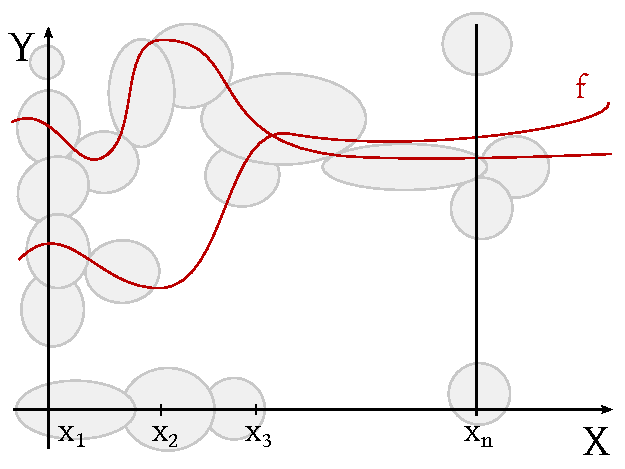
\includegraphics{img/covering.pdf}
							\caption{Covering of a function graph}
							\label{img:cov}
						\end{center}
					\end{figure}

					Now, for each tuple of indices $(y_{1,j_1}, \dots, y_{n,j_n})$ define $f_{y_{1,j_1}, \dots, y_{n,j_n}} \in \mathcal C(x, y)$ to be such that $f_{y_{1,j_1},\dots,y_{n,j_n}}(x_i) \in B_{\frac\varepsilon4}(y_{i,j_i})$ if such an $f$ exists. The set $F$ of all such functions is finite. We show that $M \subset \bigcup_{q \in F} B_{\varepsilon}(q)$.

					Take $f \in M$ arbitrary. Now choose $\alpha = (y_{1,j_1}, \dots, y_{n,j_n})$ such that $f(x_i) \in B_{\frac\varepsilon4}(y_{i,j_i})$ and pick $f_\alpha \in F$ accordingly.

					Take $x \in X$ arbitrary and $x_i$ such that $x \in B_\delta(x_i)$
					\begin{align*}
						\implies d(f(x), f_\alpha(x)) &\leq d(f(x), f(x_i)) + d(f(x_i), f_\alpha(x_i)) + d(f_\alpha(x_i), f_\alpha(x)) \\
							&< \frac\varepsilon4 + \frac\varepsilon2 + \frac\varepsilon4 = \varepsilon \\
						\implies d_C(f, f_\alpha) &= \sup_{x \in X} d(f(y), f_\alpha(x)) < \varepsilon
					\end{align*}
			\end{description}
	\end{enumerate}
\end{proof}

\begin{Remark}
	Compare this to the fact that $B_1(0)$ in $C(X, Y)$ is \emph{not} compact.
\end{Remark}

To complete this chapter, we discuss an important topological assertion; the Baire category theorem.

\begin{Remark}[Motivation]
	In general, let $(X, d)$ be a metric space. Let $A$ and $B$ be open and dense, then also $A \cap B$ is dense.
\end{Remark}

\begin{proof}
	Show $\forall x \in X \forall \varepsilon: B_\varepsilon(x) \cap [A \cap B] = \emptyset$.
	Take $x \in Y, \varepsilon > 0 \implies \exists x_1 \in B_{\varepsilon}(x) \cap A$. $A$ is dense.
	$A$ is open, so $\exists \varepsilon > 0: B_{\varepsilon_1}(x_1) \subset B(x) \cap A$.
	$B$ is dense, so $B_{\varepsilon_1}(x_1) \cap X \neq \emptyset$.
	\[ \implies \exists z \in B_{\varepsilon}(x_1) \cap B \]
	\[ B_{\varepsilon_1}(x_1) \subset B(x) \cap A \implies z \in B_\varepsilon(x) \cap (A \cap B) \]
\end{proof}

More generally, $\forall A_1, \dots, A_n$ open, dense $\implies \bigcap_{i=1}^n A_i$ is dense (this is left as an exercise).
Does this also hold true for countably many $A_i$?

\begin{theorem}[Baire theorem]
	\label{theorem:1.23}
	\index{Baire theorem}
	Let $(X, d)$ be a complete metric space.
	Let $\left(O_n\right)_{n \in \mathbb N}$ be a sequence of dense sets.
	Then $\bigcap O_n$ is dense.
\end{theorem}
\begin{proof}
	Let $D \coloneqq \bigcap_{n \in \mathbb N} O_n$. Show that for $x \in X$, $\varepsilon > 0$ arbitrary we have $B_{\varepsilon}(x) \cap D \neq \emptyset$.
	We define iteratively a sequence $(x_n)_{n \in \mathbb N}$.

	\begin{description}
		\item[$\mathbf{n = 1}$] Take $x_1, \varepsilon_1$ such that
			\[ \overline{B_{\varepsilon_1}(x_1)} \subset O_1 \cap B_{\varepsilon}(x) \text{ with } \varepsilon_1 < \frac\varepsilon2 \]
		\item[$\mathbf{n-1\to n}$] Given $x_{n-1}, \varepsilon_{n-1}$, take $x_n, \varepsilon_n$ such that
			\[ \overline{B_{C_n}(x_n)} \subset O_n \cap B_{\varepsilon_{n-1}}(x_{n-1}) \quad \text{ and} \quad \varepsilon_n < \frac{\varepsilon_{n-1}}{2} \]
	\end{description}

	This provides sequences $(x_n)_n, (\varepsilon_n)_n$ such that $\varepsilon_n < \frac\varepsilon{2^n}$ and $x_n \in B_{\varepsilon_N}(x_N) \forall n \geq N$
	\[ \implies (x_n)_n \text{ is Cauchy, } X \text{ complete } \implies \exists x \in X: x_n \to x \]
	\[ \text{ since } x_n \in \overline{B_{\varepsilon_N}}(x_N) \forall n \geq N \implies x \in \overline{B_{\varepsilon_N}(x_n)} \implies x \in D \cap B_{\varepsilon}(x) \]
\end{proof}

We consider a common, but less useful reformulation:

\begin{definition}
	\label{defintion:1.24}
	Let $(X, d)$ be a metric space, $M \subset X$. We say
	\begin{itemize}
		\item $M$ is \emph{nowhere dense}\index{Nowhere dense}\dt{nirgends dicht}, if $\mathring{\overline M} = \emptyset$
		\item $M$ is of \emph{first category}\index{Set of first category}\index{First category} $\iff M$ is a countable union of nowhere dense sets
		\item $M$ is of \emph{second category}\index{Set of second category}\index{Second category} $\iff M$ is not of first category
	\end{itemize}
\end{definition}

\begin{theorem}[Baire category theorem (weaker version)]
	\index{Baire theorem}
	Let $(X, d)$ be a complete metric space. Then $(X, d)$ is of second category.

	In other words (which is a useful formulation):
	If $X = \bigcup_{n \in \mathbb N} C_n \implies \exists n_0: \mathring{\overline C} \neq \emptyset$.
	In particular, if
	\[ X = \bigcup_{n \in \mathbb N} C_n \text{ with } C_n \text{ closed } \implies \exists n_0: \mathring{C_{n_0}} \neq \emptyset \]
\end{theorem}

\begin{proof}
	Suppose that $X = \bigcup_{n \in \mathbb N} O_n = \bigcup_{n \in \mathbb N} \overline{O_n}$ with $\mathring{\overline O_n} = \emptyset \forall n$
	\[ \mathring{\overline O}_n = \emptyset \implies \overline{\overline{O}_n^C} = X \]
	Why does this implication hold? Because consider $x \in X, \varepsilon > 0$.
	\[ B_\varepsilon(x) \cap \overline O_n^C = \emptyset \implies B_{\varepsilon}(x) \subset \overline{O}_n \implies \mathring{\overline O_n} \neq \emptyset \text{ hence } B_\varepsilon(x) \cap {\overline O}_n^C \neq \emptyset \]
	Okay, then we continue by the conclusion \dots
	\[ \implies \overline{O_n}^C \text{ is open and dense } \forall n \xrightarrow{\text{Theorem~\ref{theorem:1.23}}} \bigcap_{n \in \mathbb N} \overline{O}_n^C \text{ is dense} \]
	\[ \bigcap_{n \in \mathbb N} \overline{O}_n^C = \left(\bigcup_{n \in \mathbb N} \overline{O}_n\right)^C = X^C = \emptyset \]
	gives a contradiction
\end{proof}

\begin{Remark}
	\begin{enumerate}
		\item This is a fundamental theorem in Functional Analysis
		\item This can be used to show that continuous, nowhere differentiable functions exist (construction is left as an exercise, e.g. Weierstrass function)
	\end{enumerate}
\end{Remark}

\section{Normed space}
\label{section:2}
\subsection{Fundamentals}
\label{section:2.1}

\begin{definition}
	\label{definition:2.1}
	Let $X$ be a vector space. A function $\Norm{\cdot}: X \to [0, \infty)$ is called \emph{seminorm}\index{Seminorm} if
	\begin{itemize}
		\item $x = 0 \implies \Norm{x} = 0$
		\item $\Norm{\lambda x} = \Abs{\lambda} \Norm{x} \forall x \in X, \lambda \in \mathbb K$
		\item $\Norm{x + y} \leq \Norm x + \Norm y \forall x, y \in X$
	\end{itemize}
	The first property differs between a norm and a seminorm.

	The tuple $(X, \Norm{\cdot})$ is called a \emph{semi-normed space}\index{Semi-normed space}.
	We transfer the notions of convergence of sequences, Cauchy sequences and completeness verbatim to semi-normed spaces.
\end{definition}

\begin{Example}[Not done in lecture]
	We found the following examples while studying:
	\[ f \text{ linear}, x \mapsto \Abs{f(x)} \qquad \text{ and } \qquad \Norm{\begin{pmatrix} x \\ y \end{pmatrix}} \coloneqq \Abs{y} \]
\end{Example}

\begin{definition}[Definition and proposition]
	\label{definition:2.2}
	Let $(X, \Norm{\cdot})$ be a semi-normed space and $(x_n)_n$ be a sequence in $X$. We say that
	\begin{itemize}
		\item $\sum_{n=1}^\infty x_n$ \emph{converges}\index{Convergence in semi-normed spaces} to $x \in X$ and write $x = \sum_{n=1}^\infty x_n$ if $\lim_{m\to\infty} \sum_{n=1}^m x_n = x$
		\item $\sum_{n=1}^\infty x_n$ is \emph{absolutely convergent}\index{Absolutely convergent} if $\sum_{n=1}^\infty \Norm{x_n}$ converges [$\iff \left(\sum_{n=1}^m \Norm{x_n}\right)_m$ is bounded]
	\end{itemize}
	It holds that $X$ is complete iff any absolutely converging series converges.
\end{definition}

\begin{proof}
	\begin{description}
		\item[$\implies$]
			Take $m_1 < m_2$ arbitrary, then
			\[ \Norm{\sum_{n=1}^{m_1} x_n - \sum_{n=1}^{m_2} x_n} \leq \sum_{n=m_1+1}^{m_2} \Norm{x_1} = \sum_{n=1}^{m_1} \Norm{x_n} - \sum_{n=1}^{m_2} \Norm{x_1} \leq \Norm{\sum_{n=1}^{m_1} \Norm{x_n} - \sum_{n=1}^{m_2} \Norm{x_1}} \]
			\[ \implies \left(\sum_{n=1}^m x_n\right)_m \text{ is Cauchy } \implies \text{ convergent} \]
		\item[$\impliedby$]
			Let $(x_n)_n$ be Cauchy. Show that $(x_n)_n$ converges. For $\varepsilon_k = 2^{-k}$, pick $N_k$ such that $\Norm{x_n - x_m} \leq 2^{-k} \forall n, m \geq N_k$
			\[ \implies \exists (x_{n_k})_k \text{ a subsequence such that } \Norm{x_{n_{k+1}} - x_{n_k}} \leq 2^{-k} \]
			Define $y_k \coloneqq x_{n_{k-1}} - x_{n_k} \implies \sum_k \Norm{y_{n_w}} \leq \sum_k 2^{-k} < \infty$
			\[ \implies \exists y \in X: \sum_{k=1}^n y_k \to y \text{ as } n \to \infty \]
			\[ \sum_{k=1}^n y_k = x_{n_{m+1}} - x_{n_1} \implies x_{n_{m+1}} \to y - x_{n_1} \text{ as } n \to \infty \]
			So $(x_n)_n$ has a convergent subsequence and $(x_n)_n$ is Cauchy, then $(x_n)_n$ is convergent.
	\end{description}
\end{proof}

\begin{Remark}
	In $\mathbb R^n$, $\sum_n x_n$ is absolutely convergent iff every permutation converges.
	In general Banach spaces, only the direction $\implies$ is true.
\end{Remark}

\dateref{2019/03/28}

\begin{proposition}[Proposition and definition]
	\label{proposition:2.3}
	Let $X$ be a vector space and $\Norm{\cdot}_1$ and $\Norm{\cdot}_2$ be two norms on $X$.
	We say $\Norm{\cdot}_1$ and $\Norm{\cdot}_2$ are equivalent if
	\[ \exists m, M > 0 \forall x \in X: m \Norm{x}_1 \leq \Norm{x}_2 \leq M \Norm{x}_1 \]
	TFAE:
	\begin{enumerate}
		\item $\Norm{\cdot}_1$ and $\Norm{\cdot}_2$ are equivalent.
		\item For any sequence $(x_n)_n$ and $x \in X, x_n \to x$ with respect to $\Norm{\cdot}_1 \iff x_n \to x$ with respect to $\Norm{\cdot}_2$
		\item For any sequence $(x_n)_n$ we have,
			\[ x_n \to 0 \text{ with respect to } \Norm{\cdot}_1 \iff x_n \to 0 \text{ with respect to } \Norm{\cdot}_2 \]
	\end{enumerate}
\end{proposition}

\begin{proof}
	$(1) \implies (2) \implies (3)$ is immediate.

	It remains to show that:
	\begin{description}
		\item[$(3) \implies (1)$] 
			Suppose no $M > 0$ exists such that $\Norm{x}_2 \leq M \cdot \Norm{x}_1 \forall x \in X$.
			\[ \implies \forall n \in \mathbb N \exists x_n \in X: \Norm{x_n}_2 > n \Norm{x_n}_1 \]
			Let $y_n \coloneqq \frac{x_n}{\Norm{x_n}_1 n}$. Then $\Norm{y_n}_1 = \frac1n \to 0$ hence $y_n \to 0$,
			but $\Norm{y_n}_2 > n \Norm{y_n}_1 = 1$.
			\[ \implies y_n \not\to 0 \text{ with } \Norm{\cdot}_2 \]
			This gives a contradiction.

			The second estimate is left as an exercise.
	\end{description}
\end{proof}

\begin{Remark}
	If $\dim(X) < \infty$, then any two norms on $X$ are equivalent.
\end{Remark}

\begin{definition}[Quotient spaces]
	\label{definition:2.4}
	Let $(X, \Norm{\cdot})$ be a normed space and $Y \subset X$ a subspace.
	Define a relation \enquote{$\sim$} on $X$ with $x \sim y :\iff x - y \in Y$.

	Then $\sim$ defines an equivalence relation on $X$.
	We define
	\begin{itemize}
		\item $[X]_\sim = \SetDef{y \in X}{x \sim y}$ is the \emph{equivalence class}\index{Equivalence class} of $x \in X$
		\item $X/Y \coloneqq \SetDef{[x]_\sim}{x \in X}$ is the \emph{quotient space}\index{Quotient space}
		\item $\pi: \begin{cases} X \to X / y \\ x \mapsto [x]_\sim \end{cases}$
	\end{itemize}

	Defining $[x] + [y] \coloneqq [x + y]$
	\[ \lambda [x] \coloneqq [\lambda x] \qquad \hat 0 \coloneqq [0] \]
	We get that:
	\begin{enumerate}
		\item $X/Y$ is a vector space
		\item $\Norm{[x]}_{X/Y} \coloneqq \inf_{y \in [x]} \Norm{y}_X$ is a semi-norm.
		\item If $Y$ is closed, then $\Norm{\cdot}_{X/Y}$ is a norm.
		\item If $X$ is complete and $Y$ closed, then $(X/Y, \Norm{\cdot}_{X/Y})$ is a Banach space.
	\end{enumerate}
\end{definition}

\begin{proof}
	\begin{itemize}
		\item Equivalence relation
		\item Vector space with \enquote{+} and \enquote{$\lambda[x]$} are well-defined
	\end{itemize}
	This is left as an exercise to the reader.

	\begin{itemize}
		\item[2.]
			\begin{itemize}
				\item 
					First of all, $\Norm{\cdot}_{X/Y} \geq 0$ is trivial.
					\[ \Norm{[0]}_{X/Y} \underbrace{=}_{\text{since } [0] = Y} \inf_{y \in Y} \Norm{Y} \leq \Norm{0} = 0 \]
				\item
					Secondly, consider $\lambda \in \mathbb K$, $[x] \in X/Y$.

					Show that: $\Norm{\lambda [x]}_{X/Y} = \Abs{\lambda} \Norm{[x]}_{X/Y}$.

					Trivial, if $\lambda = 0$. Assume $\lambda \neq 0$,
					\[ \Norm{\lambda [x]}_{X/Y} = \Norm{[\lambda x]}_{X/Y} = \inf_{y \in [\lambda x]} \Norm{y} = \inf_{y \in X, \frac y\lambda \in [x]} \Norm{y} = \inf_{w \in [x]} \Norm{\lambda w} = \Abs{\lambda} \overbrace{\inf_{u \in [x]} \Norm{u}}^{\Norm{[x]}_{X/Y}} \]

				\item Take $[x_1], [x_2] \in X/Y, \varepsilon > 0$.
					We note that
					\[ \Norm{[x]}_{X/Y} = \inf_{\substack{y \in X \\ w \in Y \\ w \coloneqq x \cdot y}} \Norm{y} = \inf_{w \in Y} \Norm{x - w} \]
					Hence we can take $y_1, y_2 \in Y$ such that $\Norm{x_1 - y_i} < \Norm{[x_i]}_{X/Y} + \varepsilon \qquad \varepsilon \in [1, 2)$.
					\begin{align*}
						\implies \Norm{[x_1] + [x_2]}_{X/Y} &= \Norm{[x_1 + x_2]}_{X/Y} \leq \Norm{x_1 + x_2 - (y_1 + y_2)} \\
							&\leq \Norm{x_1 - y_1} + \Norm{x_2 - y_2} \leq \Norm{[x_1]}_{X/Y} + \Norm{[x_2]}_{X/Y} + 2 \varepsilon
					\end{align*}
					Since $\varepsilon$ was arbitrary, the assertion follows.
			\end{itemize}
		\item[3.] Suppose $Y$ is closed if $\Norm{[x]}_{X/Y} = 0$, then
			\[ \inf_{y \in Y} \Norm{x - y} = 0 \implies \exists (y_n)_n \text{ in } Y \text{ s.t. } \lim_{n \to \infty} \Norm{x - y_n} = 0 \]
			\[ Y \text{ closed } \implies x \in Y \implies [x] = [0] = \hat 0 \]
		\item[4.] Take $([x_n])_n$ to be a sequence in $X/Y$ and suppose that $\sum_{i=1}^\infty \Norm{[x_n]}_{X/Y} < \infty$. If we can show that $\exists [x] \in X/Y$ such that $\sum_{i=1}^\infty [x_n] = [x]$, then by Proposition~\ref{definition:2.2}, $X/Y$ is complete.

			Choose $\forall n \in \mathbb N: \tilde x_n \in [x_n]$ such that $\Norm{\tilde x_n} \leq \Norm{[x_n]}_{X/Y} + 2^{-n}$
			\[ \implies \sum_{n=1}^\infty \Norm{\tilde x_n} \leq \sum_{n=1}^\infty \left(\Norm{[x_n]}_{X/Y} + 2^{-n}\right) < c < \infty \]
			\[ X \text{ complete} \implies \exists x \in X: \sum_{n=1}^\infty \tilde x_n = x \qquad \Norm{[x] - \sum_{n=1}^m \underbrace{[x_n]}_{[\tilde x_n]}}_{X/Y} \leq \Norm{x - \underbrace{\sum_{k=0}^n \tilde x_k}_{\to 0}} \]
	\end{itemize}
\end{proof}

\dateref{2019/04/02}

\begin{corollary}
	\label{corollary:2.5}
	Let $X$ be a vector space with semi-norm $\Norm{\cdot}_X: X \to [0, \infty)$. Then
	\begin{itemize}
		\item $N = \SetDef{x \in X}{\Norm{x}_X = 0}$ is a subspace at $X$
		\item $\Norm{[X]} \coloneqq \Norm{X}_p$ is a norm on $X/N$
		\item If $X$ is complete, then $(X/N, \Norm{\cdot})$ is a Banach space.
	\end{itemize}
\end{corollary}

\begin{proof}
	The proof is left as an exercise.
\end{proof}

\begin{proposition}
	\label{proposition:2.6}
	Let $(X, \Norm{\cdot})$ be a normed space, $U \subset X$ is a subspace. Then
	\begin{itemize}
		\item $\overline{U}$ is also a subspace.
		\item $X$ is separable iff $\exists A \subset X$ complete such that $X = \overline{\mathcal L(A)}$ where $L(A) = \SetDef{\sum_{i = 1}^n \lambda_i x_i}{x_i \in A, \lambda_i \in \mathcal K, n \in \mathbb N}$
	\end{itemize}
\end{proposition}

\begin{proof}
	\begin{itemize}
		\item Left as an exercise
		\item
			\begin{description}
				\item[$\implies$] True since $\exists A \subset X$ countable such that $\overline{A} = X \implies \underline{X} = \overline{A} \subset \overline{L(A)} \subset X$
				\item[$\impliedby$] Let $A \subset X$ countable such that $\overline{\mathcal L(A)} = X$. Define
					\[ B = \SetDef{\sum_{i = 1}^n (\lambda_i + i \mu_i) x_i}{\lambda_i, \mu_i \in \mathbb X, x \in A, n \in \mathbb N} \]
					where $i$ is the imaginary unit if $\mathbb K = \mathbb C$ or $i = 0$ if $\mathbb K = \mathbb R$.
					Then $B$ is countable.

					Show: $\forall x \in X \forall \varepsilon \exists x \in B: \Norm{x - y} < \varepsilon$.

					Take $x \in X, \varepsilon > 0 \implies \exists x_0 \in \mathcal L(A): \Norm{x - x_i} < \frac\varepsilon2$ when $x_0 = \sum_{i = 0}^n (\lambda_i + i \mu_i) x_i$ with $\lambda_i, \mu_i \in \mathbb R, x_i \in A$.
					Choose $\lambda', \mu_i' \in \mathbb Q$ such that
					\[ \sqrt{(\lambda_i - \lambda_i')^2 + (\mu_i - \mu_i')^2} \leq \frac{\varepsilon}{L \cdot \sum_{i = 1}^n \Norm{x_i}} \forall i \in \Set{1, \dots, n} \]
					Let $y \coloneqq \sum_{j=1}^n (\lambda_i' + \mu_i')x_i \subset B$.
					\begin{align*}
						\implies \Norm{x - y} &\leq \Norm{x - x_0} + \Norm{x_0 - y}
							&\leq \frac{\varepsilon}{2} \\
							&\leq \sum_{i=1}^n \Abs{(\lambda_i + i \varepsilon_i) - (\lambda_i' + i \mu_i')} \Norm{x_i} \\
							&\leq \frac{\varepsilon}{2} + \sum_{i = 1}^n \Norm{x_i} \cdot \frac{\varepsilon}{2 \sum_{i=1}^n \Norm{x_i}} = \varepsilon
					\end{align*}
			\end{description}
	\end{itemize}
\end{proof}

\begin{proposition}[Proposition and definition]
	\label{proposition:2.7}
	Let $(X, \Norm{\cdot}_{x_i})$ for $i = 1, \dots, n$ be a normed space. Denote by
	\[ X_1 \otimes X_1 \otimes \ldots \otimes X_n = \bigotimes_{i=1}^n X_i = X_1 \times \dots \times X_n = \SetDef{(x_1, \dots, x_n)}{x_i \in X_i, i = 1, \dots, n} \]
	For $p \in [1, \infty]$, define
	\[
		\Norm{(x_1, \dots, x_n)}_{\otimes_i X_i, p}
		= \begin{cases}
			\left(\sum_{i=1}^n \Norm{x_i}_{x_i}^p\right)^{\frac1p} & \text{if } p \in [1, \infty] \\
			\max_{i=1,\dots,n} \Norm{x_i}_{x_i} & \text{if } p = \infty
		\end{cases}
	\]
	Then
	\begin{itemize}
		\item $(\bigotimes_{i} X_i, \Norm{\cdot}_{\bigotimes_i X_i, p})$ is a normed space with respect to componentwise addition and multiplication.
		\item If all $X_i$ are complete, then $\bigotimes_{i=1}^n X_i$ is complete.
		\item All norms $\Norm{\cdot}_{\bigotimes_{i} X_i, p}$ are equivalent.
	\end{itemize}
\end{proposition}

\begin{proof}
	\begin{itemize}
		\item Vector space properties: Left as an exercise
		\item Norm: $\Norm{x}_{\bigotimes_{i} X_i, n} = 0 \iff x = 0$ \\
			$\Norm{\lambda x}_{\bigotimes_{i} X_i, p} = \Abs{\lambda} \Norm{x}_{\bigotimes_{i} X_i, p}$
		\item Triangle inequality: $p = 1$, $p = \infty$ \\
			$p \in (1, \infty)$. Take $x, y \in \bigotimes_{i=1}^n X_i$ and we write $\Norm{\cdot}_p = \Norm{\cdot}_{\bigotimes_i X_i,p}$.
			\begin{align*}
				\implies \Norm{x + y}_p^p
					&= \sum_{i=1}^n \Norm{x_i + y_i}_{X_i} \Norm{x_i + y_i}_{x_i}^{p-1} \\
					&\leq \sum_{i=1}^n \Norm{x_i}_{X_i} \Norm{x_i + y_i}_{X_i}^{p-1} + \sum_{i=1}^n \Norm{y_i}_{X_i} \Norm{x_i + y_i}^{p-1}_{X_i} \\
					&\underbrace{\leq}_{\substack{\text{Hölder} \\ \text{ineq.}}} \left(\sum_{i=1}^n \Norm{X_i}_{X_i}^p\right)^{\frac1p} \cdot \left(\sum_{i=1}^n \Norm{x_i + y_i}_{X_i}^{(p-1)q}\right)^{\frac1q} \\
					&\qquad+ \left(\sum_{i=1}^n \Norm{y_i}_{x_i}^p\right)^{\frac1p} \left(\sum_{i=1}^n \Norm{x_i + y_i}^{(p-1)q}\right)^{\frac1q} \\
					&= \Norm{x}_p \Norm{x + y}_p^{p-1} + \Norm{y}_p \Norm{x + y}_p^{p-1} \\
					&= \left(\Norm{x}_p + \Norm{y}_p\right) \cdot \Norm{x + y}_p^{p-1} \\
			\end{align*}%
			%
			%+ \left(\sum_{i=1}^n \Norm{y_i}_{X_i}^p)^{\frac1p} \left(\Norm{x_i + y_i}^{(p-1)q}\right)^{\frac1q}
			%= \Norm{x}_p \Norm{x + y}_p^{p+1} + \Norm{y}_p \Norm{x + y}_p^{p-1}
			%
			\[ \implies \Norm{x + y}_p \leq \Norm{x}_p + \Norm{y}_p \text{ if } x + y \neq 0 \: (\text{trivial otherwise}) \]

			Completeness, equivalence is trivial to show (left as an exercise) (use norm equivalence in $\mathbb R^n$)
	\end{itemize}
\end{proof}

\begin{definition}
	\label{definition:2.8}
	Let $(X, \Norm{\cdot}_X)$ and $(Y, \Norm{\cdot}_Y)$ be normed spaces. If $j: X \to Y$ is linear such that $\Norm{j(x)}_Y = \Norm{x}_X$ (hence $j$ is injective) then $j$ is called isometric embedding from $X$ to $Y$. If $j$ is bijective, then $j$ is called \emph{isometric isomorphism}\index{Isometric isomorphism} and we say $X = Y$ up to isomorphism.
\end{definition}

\begin{proposition}
	\label{proposition:2.9}
	Let $(X, \Norm{\cdot}_X)$ be a normed space. Then $\exists (\hat X, \Norm{\cdot}_X)$ a Banach space such that
	\begin{enumerate}
		\item $\exists$ isometric embedding, $i: X \to \hat X$ such that $\overline{j(X)} = \hat X$ [$\hat X$ can be regarded as completion of $X$]
		\item If $j_1: X \to Y$ is an isometric embedding on $Y$, a Banach space
			\[ \implies \exists i_2: \hat X \to Y \]
			an isometric embedding such that $j_2 \circ j = j_1$ and if $\overline{j_1(x)} = Y$ then $j_2$ is an isometric isomorphism.
			Thus \enquote{the completion is essentially unique}.
	\end{enumerate}
\end{proposition}

\begin{proof}
	\begin{enumerate}
		\item 
			Set $\hat X = \SetDef{(x_n)_n}{x_n \in X \forall n, (x_n)_n \text{ is } Cauchy}$. $\hat X$ is a vector space by
			\[ (x_n)_n + (y_n)_n \coloneqq (x_n + y_n)_n \qquad \lambda (x_n)_n \coloneqq (\lambda x_n)_n \quad \hat 0 \coloneqq (0)_n \]
			Define $\Norm{(x_n)_n}_{\tilde X} \coloneqq \lim_{n \to \infty} \Norm{x_n}$ [well-defined since $(\Norm{x_n})_n$ is Cauchy in $\mathbb R$].
			Then $\Norm{\cdot}_{\tilde X}$ is a semi-norm (proof is left as an exercise).
			Setting $N = \SetDef{(X_n)_n}{\Norm{(X_n)_n}_{\hat X} = 0}$. By Corollary~\ref{corollary:2.5}, $\hat X \coloneqq \hat X \setminus N$ with $\Norm{[(X_n)_n]}_{\hat X} = \Norm{(X_n)_n}_{\hat X}$ is a normed space. Define
			\[ j: X \to \hat X \qquad x \mapsto [(x)_n] \]
			then $j$ is linear and $\Norm{j(x)}_{\hat x} = \Norm{[(x)_n]}_{\hat x} = \lim_{n \to \infty} \Norm{x} = \Norm{x}$.
			So $j$ is an isometric embedding.

			Show: $\overline{j(X)} = \hat{X}$.

			Take $\hat x = [(X_n)_n] \in \hat X$. Define $y_n \coloneqq j(x_n) \in \hat X$.
			\begin{align*}
				\implies \Norm{y_m - [(x_n)_n]}_{\hat X}
					&= \Norm{(x_m)_n - (x_n)_n}_{\hat X} = \lim_{n \to \infty} \Norm{x_m - x_n} \\
					&= \lim_{n \geq n_0} \Norm{x_m - x_n} < \varepsilon
			\end{align*}
			Now, $\forall \varepsilon > 0 \exists n \forall n, m \geq n_0: \Norm{x_n - x_m} < \varepsilon$.

			Show: $\hat X$ is complete.

			Let $(y_n)_n$ be Cauchy in $\hat X$. Pick $X_n \in X$ such that $\Norm{j(x_n) - y_n}_{\hat X} \leq \frac 1n$ ($\overline{j(x)} = \hat x$)
			\begin{align*}
				\implies \Norm{x_n - x_m}_X = \Norm{j(x_n) - j(x_m)}_{\hat X}
					&\leq \Norm{j(x_n) - y_n}_{\hat X} + \Norm{y_n - y_m}_{\hat X} + \Norm{y_n - j(x_n)}_{\hat X}
			\end{align*}
			Take $\varepsilon > 0$. Then $\exists n_0 \forall n, m \geq n_0: \Norm{y_n - y_m}_{\hat X} < \frac\varepsilon3$.
			Pick $n_1$ such that $\forall n \geq n_1: \frac1n < \frac{\varepsilon}{100}$.
			\[ \implies \forall n, m > \max(n_0, n_0): \Norm{x_n - x_m} \leq \frac{\varepsilon}{100} + \frac{\varepsilon}{3} + \frac{\varepsilon}{100} < \varepsilon \]
			$\implies (x_n)_n$ is Cauchy. Let $y \coloneqq (X_n)_n \in \tilde X$.
			Then
			\[ \Norm{y_n - [y]}_{\hat X} \leq \Norm{y_n - j(x_n)}_{\hat X} + \Norm{j(x_n) - [y]}_{\hat X} \leq \frac1n + \lim_{n \to \infty} \Norm{x_n - x_m}_X \xrightarrow{n \to \infty} 0 \]

		\item
			\dateref{2019/04/04}
			Let $\hat x \in \hat X \implies \exists (x_n)_n \in X$ such that $j(x_n) \to \hat x \implies \Norm{x_n - x_m}_X = \Norm{j(x_n) - j(x_m)}_{\hat X}$.
			\begin{itemize}
				\item[$\implies$] $(x_n)_n$ is a Cauchy sequence.
				\item[$\implies$] $j_1(x_n)$ is a Cauchy sequence in $Y$.
				\item[$\implies$] $\exists \lim_{n \to \infty} j_1(x_n) \coloneqq y$
			\end{itemize}
			Using this, we define $j_2: \hat X \to Y$ with $\hat x \mapsto \lim_{n \to \infty} j_1(x_1)$ where $j(x_1) \to \hat x$.

			Well-defined? Take $\hat x \in \hat X$ and $j(x_n) \to \hat x$, $j(y_n) \to \hat x$.
			\[ \implies \Norm{i_1(x_n) - j_1(y_n)} = \Norm{x_n - y_n} = \Norm{j(x_n) - j(y_n)} \to 0 \text{ as } n \to \infty \]
			\[ \implies \lim_{n \to \infty} j_1(x_n) = \lim_{n \to \infty} j_1(y_n) \implies j_1 \text{ well-defined} \]

			Show linearity is left as an exercise. By isometry, take $\hat x \in \hat X$,
			\[ \Abs{i_2(\hat x)} \underbrace{=}_{j(x_n) \to \hat x} \lim_{n \to \infty} \Norm{j_1(x_1)} = \lim_{n \to \infty} \Norm{x_n} = \lim_{n \to \infty} \Norm{i(x_n)} = \Norm{\hat x} \]

			Show: $j_2 \circ j = j_1$. Take $x \in X \implies (x_n)$ is such that $j(x) \to j(x) \implies j_2(j(x)) = \lim_{n \to \infty} j_1(x) = j_1(x)$.

			Assume that $\overline{j_1(x)} = Y$. Take $y \in Y$. Find $\hat x \in \hat X$ such that $i_2(\hat x) = y$.
			By $\overline{j_1(x)} = Y \implies \exists (x_n)_n \text{ in } X$ such that $i_1(x_n) \to Y \implies (j_1(x_n))_n$ is Cauchy.
			\[ \implies (x_n)_n \text{ Cauchy } \implies (j(x_n))_n \text{ is Cauchy} \]
			\[ \xRightarrow{\hat X \text{ complete}} \exists \hat x \text{ such that } \lim_{n \to \infty} j(x_n) = \hat x \implies j_2(\hat x) = \lim_{n \to \infty} j_2(x_n) = Y \]
	\end{enumerate}
\end{proof}

\subsection{Important examples of normed spaces}
\label{section:2.2}

\begin{definition}[Basic notation]
	\label{definition:2.10}
	Let $\Omega \subset \mathbb R^N$, $f: \Omega \to \mathbb K^M$ with $N, M \subset \mathbb N$.
	\begin{itemize}
		\item We call $\Omega$ a \emph{domain}\index{Domain}\dt{Gebiet} if $\Omega$ is open and connected, where connected means that $\forall x, y \in \Omega$ there is a curve in $\Omega$ connecting $X$ and $Y$.
		\item For $\alpha = (\alpha_1, \dots, \alpha_N) \in \mathbb N_0^N$ define $\Abs{\alpha} = \alpha_1 + \alpha_2 + \dots + \alpha_N$. If $f$ is $r$-times continuously differentiable, we set for $\alpha \in \mathbb N_0^N$, $\Set{\alpha} \leq r$.
		\[ D^\infty f \coloneqq \frac{\partial^{\alpha_1} \dots \partial^{\alpha_n}}{\partial_{x_1}^{\alpha_1} \dots \partial_{x_n}^{\alpha_n} x_n} f \]
		where $\frac{\partial^{\alpha_1}}{\partial^{\alpha_i} x_i}$ is the partial derivative of $f$ with respect to $x_i$ of order $\alpha_i$.

		\begin{example}
			Let $N=2$ and $\alpha = (1, 1)$.
			\[ D^\infty f = \frac{\partial^{\alpha_1}}{\partial x_1} \frac{\partial^{\alpha_2}}{\partial x_2} f \]
			Let $\alpha = (2, 0)$.
			\[ D^\infty f = \frac{\partial^{\alpha_1}}{\partial^2 x_1} f \]
		\end{example}
	\end{itemize}

	\begin{itemize}
		\item For $z \in \mathbb K^N$ we denote $\Abs{z} \coloneqq \sqrt{\sum_{i=1}^N \Abs{z_i}^2}$.\footnote{This is an abuse of notation with $\Abs{\alpha}$ for $\alpha \in \mathbb N_0^N$}
		\item We say $E \subset \Omega$ is compact in $\Omega$ and we write $E \Subset \Omega$ if $E$ is compact.
			\begin{Remark}
				If $E \Subset \Omega$, then $\exists \delta > 0: \inf\SetDef{\Norm{x - y}}{x \in E, y \in \partial \Omega} > 0$.
			\end{Remark}
			\begin{proof}
				Left as an exercise (use compactness)
			\end{proof}
		\item $f$ is \emph{compactly supported}\index{Compactly supported} in $\Omega$ if $\operatorname{supp}(f) \ll \Omega$.
		\item $\operatorname{supp}(f) \coloneqq \overline{\SetDef{x \in \Omega}{\Norm{f(x)} > 0}}$
	\end{itemize}
\end{definition}

\dateref{2019/04/09}

\begin{definition}[Definition and proposition, Spaces of continuous functions]
	\label{definition:2.11}
	Let $\Omega \subset \mathbb R^N$ be a domain. We define
	\begin{align*}
	  C_b(\Omega, \mathbb K^M) &= \SetDef{\varphi: \Omega \to \mathbb K^M}{\varphi \text{ bounded}} \text{ with } \Norm{\varphi}_{C_b} = \Norm{\varphi}_\infty = \sup_{x \in \Omega} \Abs{\varphi(x)} \\
	  C(\overline\Omega, \mathbb K^M) &= \SetDef{\varphi: \Omega \to \mathbb K^M}{\varphi \text{ can be continuously extended to } \overline\Omega}, \Norm{\varphi}_C \coloneqq \Norm{\varphi}_\infty \\
	  C^r(\overline\Omega, \mathbb K^M) &= \SetDef{\varphi: \Omega \to \mathbb K^M}{D^\alpha \varphi \in C(\overline\Omega, \mathbb K^M) \forall \alpha \in \mathbb N_0^N: \Abs{\alpha} \leq r} \text{ and} \Norm{\varphi}_{C^r} = \sum_{\substack{\alpha \in \mathbb N_0^N \\ \Abs{\alpha} \leq r}} \Norm{D^\infty \varphi}_{\infty} \\
	  C^r_C(\Omega, \mathbb K^M) &= \SetDef{\varphi: \Omega \to \mathbb K^M}{\operatorname{supp}(\varphi) \ll \Omega, \varphi \in C^r(\overline\Omega, \mathbb K^M)} \text{ and } \Norm{\varphi}_{C^r_C} = \Norm{\varphi}_{C^r} \\
	  C^\infty(\overline \Omega, \mathbb K^M) &= \bigcap_{r \in \mathbb N} C^r(\overline \Omega, \mathbb K^M) \\
	  D(\Omega, \mathbb K^M) &= C_C^\infty(\Omega, \mathbb K^M) \coloneqq \bigcap_{r \in \mathbb N} C_C^r(\Omega, \mathbb K^M), C_0^r(\Omega, \mathbb K^M) = \overline{C_C^r(\Omega, \mathbb K^M)} \text{ in } C^r(\overline{\Omega}, \mathbb K^M)
	\end{align*}
	Then for any bounded $\Omega$, $C^r, C_0^r, C_b$ are Banach spaces and $C^r_C$ is a normed space.
	
	Recall: $z \in \mathbb K^M \implies \Abs{z} \coloneqq \sqrt{\sum_{i=1}^M \Abs{z_i}^2}$
\end{definition}

\begin{proof}
	The functions $\Norm{\cdot}_{C_b}, \Norm{\cdot}_{C^r}$ are norms (proof is left as an exercise).

	Show that $C_b$ is complete: Take $(\varphi_n)_n$ in $C_b$ to be Cauchy.
	\[ \implies \forall x \in \Omega: (\varphi_n(x))_n \text{ is Cauchy in } \mathbb K^n \]
	because $\Abs{\varphi_n(x) - \varphi_m(x)} \leq \Norm{\varphi_n - \varphi_m}_\infty$.
	Hence we can define $\varphi(x) \coloneqq \lim_{n \to \infty} \varphi_n(x)$.

	Show: $\varphi_n \to \varphi$ in $\Norm{\cdot}_\infty$. Take $\varepsilon > 0$.
	Show that $\exists n_0 \forall n \geq n_0: \Norm{\varphi - \varphi_n}_\infty < \varepsilon$.
	Take $n_0$ such that $\forall n, m \geq n_0: \Norm{\varphi_n - \varphi_m}_\infty < \varepsilon$. Take $m \geq n_0$.
	\[ \implies \forall x \in \Omega: \Abs{\varphi(x) - \varphi_m(x)} = \lim_{\substack{n \to \infty \\ n \geq n_0}} \Abs{\varphi_n(x) - \varphi_m(x)} < \Norm{\varphi_n - \varphi_m}_\infty \]

	Show: $\varphi$ is bounded, i.e. $\exists C > 0: \Abs{\varphi(x)} \leq C < \Norm{\varphi_n - \varphi_m}_\varepsilon < \infty$.
	Take $n$ suchthat $\Norm{\varphi - \varphi_n}_\infty < 1$
	\[ \implies \forall x \in \Omega: \Abs{\varphi(x)} > \Abs{\varphi(x) - \varphi_n(x)} + \Abs{\varphi_n(x)} \leq 1 + \underbrace{\Norm{\varphi_n}}_{= C} \]

	Now $C^r(\overline\Omega, \mathbb K^n)$ is a subspace of $C^b(\Omega, \mathbb K^n)$.
	Also $C^r(\overline\Omega, \mathbb K^n)$ is closed, since the uniform limit of $\varphi \in C^r(\overline\Omega, \mathbb K^n)$
	with respect to $\Norm{\cdot}_{C^r}$ is again in $C^r(\overline\Omega, \mathbb K^M)$ [a result from Analysis].
	\[ \implies C^r(\overline \Omega, \mathbb K^M) \text{ is a Banach space} \]
	$C_C^r(\overline\Omega, \mathbb K^M)$ is closed by definition, hence Banach.

	$C_C^r(\Omega, \mathbb K^M)$ is a vector space, since $\forall \lambda \in \mathbb K: \varphi \in C_0^r(\Omega, \mathbb K^M): \operatorname{supp}(\lambda \varphi) = \operatorname{supp}(\varphi)$ and for $\varphi, \Psi \in C_0^r(\Omega, \mathbb K^M): \operatorname{supp}(\varphi + \Psi) \ll \Omega$.
\end{proof}

\begin{definition}[Definition and proposition]
	\label{definition:2.12}
	Let $(\Omega, \Sigma, \mu)$ with $\Omega \subset \mathbb R^N$ be a measure space (i.e. $\Sigma$ is a sigma algebra and $\mu$ is a measure).
	For $p \in [1, \infty)$, we define
	\begin{align*}
		\mathcal L^p(\Omega, \mathbb K^M, \mu)
			&= \SetDef{f: \Omega \to \mathbb K^M}{f \: \mu-\text{ measurable and } \int_\Omega \Abs{f(x)}^p d \mu(x) < \infty} \\
		\Norm{f}_p^* &= \left(\int_\Omega \Norm{f(x)}^p \, d\mu(x)\right)^{\frac1p} \\
		\mathcal L^\infty(\Omega, \mathbb K^M, \mu) &\coloneqq \SetDef{f: \Omega \to \mathbb K^M}{\exists N \in \Sigma: \mu(N) = 0 \land \sup_{x \in \Omega \setminus N} \Abs{f(x)} < \infty} \\
		\Norm{f}^*_\infty &= \inf_{\substack{N \in \Sigma \\ \mu(N) = 0}} \sup_{x \in \Omega \setminus N} \Abs{f(x)}
	\end{align*}
	Our proposition is that these are semi-norms.
\end{definition}

\begin{proof}
	Show that $\Norm{\cdot}_p^*$ for $p \in [1, \infty]$ are seminorms.
	
	They cannot be norms since $\Norm{f}_p^* = 0$ for
	\[ f(x) = \begin{cases} 1 & x \in N \\ 0 & x \not\in N \end{cases} \]
	$0 \neq N \in \Sigma, \mu(N) = 0$.
\end{proof}

\begin{proposition}[Hölder inequality]
	\label{proposition:2.13}
	Let $p \in [1, \infty]$ and
	\[ a = p^* = \begin{cases} \frac{p}{p-1} & \text{ if }  \in (1, \infty) \\ 1 & \text{ if } p = \infty \\ \infty & \text{ if } p = 1 \end{cases} \]
	\[ \frac1p + \frac1{p^*} = 1 \]
	If $f \in \mathcal L^p(\Omega, \mathbb K^M, \mu)$ and $q \in \mathcal L^q(\Omega, \mathbb K^M, \mu)$ then for both
	\begin{align*}
	  f\cdot g: \: & \Omega \to \mathbb K \text{ with } x \mapsto (f(x), g(x)) = \sum_{i=1}^M f_i(x) = \overline{g_i(x)} \\
	  f \otimes g: \: & \Omega \to \mathbb K^M \text{ with } x \mapsto (f_i(x), \varphi_i(x))_{i=1}^M
	\end{align*}
	we have that $fg \in \mathcal L^1(\Omega, \mathbb K, \mu)$ and $f \otimes g \in L^1(\Omega, \mathbb K^M, \mu)$ and $\Norm{f \otimes g}_1^* \leq \Norm{fg}_1^* \leq \Norm{f}_p^* \cdot \Norm{q}_q^*$.
\end{proposition}

\begin{proof}
	\begin{description}
		\item[Case $p \in (1, \infty)$:]
			Intermediate result: $\forall \sigma, \tau \geq 0, r \in (0, 1]: \sigma^r \tau^{1-r} \leq r \sigma + (1 - r) \tau$ [AGM-inequality].
			\begin{proof}
				\item[Case $\sigma = 0$ or $\tau = 0$:] immediate
				\item[Case $\sigma, \tau > 0$:]
					\begin{align*}
						\log(\sigma^r \tau^{1-r}) &= r \log(\sigma) + (1 - r) \log(\tau) \leq \log(r\sigma + (1 - r) \tau) \\
							& \text{ since } \log''(x) \leq 0 \text{ implies that log is concave} \\
						\log \text{ is monotonic } & \implies \sigma^r \tau^{1-r} \leq r \sigma + (1 - r) \tau
					\end{align*}
			\end{proof}

			Let $A \coloneqq \left(\Norm{f}_p^*\right)^p$ and $B \coloneqq \left(\Norm{\varphi}_1^*\right)^q$ with $r = \frac1p \in (0, 1]$
			we get
			\[ \forall x \in \Omega: \left(\frac{\Abs{f(x)}^p}{A}\right)^{\frac1p} \left(\frac{\varphi(x)}{B}\right)^{\frac1q} = \frac1p \frac{\Abs{f(x)}^p}{A} + \frac1q \frac{\Abs{q(x)}^q}{B} \]
			\[ \implies \frac{\int_\Omega \Abs{f(x)} \Abs{q(x)} \, d\mu(x)}{A^{\frac1p} B^{\frac1q}} \leq \frac1p \frac{\int_\Omega \Abs{f(x)}^p \, d\mu(x)}{A} + \frac1q \frac{\int_\Omega \Abs{q(x)}^q \, d\mu(x)}{B} \]
			\[ \implies \int_\Omega \Abs{f(x)} \Abs{g(x)} \, d\mu(x) \leq \Norm{f}_p^* \Norm{g}_q^* = \frac1p + \frac1q = 1 \]

			Now: $\Norm{f \cdot g}_x^* \leq \Norm{f}_p^* \cdot \Norm{g}_q^*$ follows since $\Abs{\IP xy} \leq \Abs x \Abs y \forall x, y \in \mathbb K^M$.

			Also:
			\[ \forall x \in \Omega: \Abs{f \otimes g(x)} = \sum_{i=1}^M \Abs{f_i(x)} \Abs{g_i(x)} = \begin{pmatrix} \Abs{f_1(x)} & \Abs{g_1(x)} \\ \vdots & \vdots \\ \Abs{f_n(x)} & \Abs{g_n(x)} \end{pmatrix}  \leq \Abs{f(x)} \Abs{g(x)} \]
			\[ \implies \int_\Omega \Abs{f \otimes g(x)} \, d \mu(x) \leq \Norm{f}_p^* \cdot \Norm{g}_q^* \]
		\item[Case $p \in \Set{1, \infty}$:]
			Without loss of generality assume that $p = 1, q = \infty$.
			$\forall N \in \Sigma \text{ with } \mu(N) = 0$ we get
			\begin{align*}
				\int_\Omega \Abs{f(x)} \Abs{g(x)} \, d\mu(x) &= \int_{\Omega \setminus N} \Abs{f(x)} \Abs{q(x)} \, \mu(x) \\
					&\leq \int_{\Omega \setminus N} \Abs{f(x)} \, d\mu(x) \cdot \sup_{x \in \Omega \setminus N} \Abs{q(x)}
					&= \int_{\Omega} \Abs{f(x)} \, d\mu(x) \cdot \sup_{x \in \Omega \setminus N} \Abs{q(x)}
			\end{align*}
			Taking the infimum over all such $N$, then
			\[ \int_\Omega \Abs{f(x)} \Abs{g(x)} \, d\mu(x) \leq \Norm{f}^*_1 \cdot \Norm{g}^*_\infty \]
			And the result follows again from $\Abs{\IP xy} \leq \Abs x \cdot \Abs y$ and componentwise $\Abs{\IP{x_i}{y_i}_i} \leq \Abs{x} \Abs{y} \forall x, y \in \mathbb K^M$
	\end{description}
\end{proof}

\begin{proposition}[Minkowski inequality]
	\label{proposition:2.14}
	For $p \in [1, \infty], f, g \in \mathcal L^p(\Omega, \mathbb K^M, \mu)$, we have that $\Norm{f + g}_p^* \leq \Norm{f}_p^* + \Norm{g}_p^*$
	with $\Norm{f}_\infty \coloneqq \inf_{\mu(N) \to 0} \sup_{x \in \Omega \setminus N} \Abs{f(x)}$.
\end{proposition}

\begin{proof}
	\begin{description}
		\item[Case $p = 1$:] trivial
		\item[Case $p \in (1, \infty)$:]
			\begin{align*}
				\left(\Norm{f + g}_p^*\right)^p
					&= \int_\Omega \Abs{f(x) + g(x)} \, d\mu(x) \\
					&= \int_\Omega \Abs{f(x)} \cdot \Abs{f(x) + g(x)}^{p-1} \, d\mu(x) \\
					&+ \int_\Omega \Abs{g(x)} \Abs{f(x) + g(x)}^{p-1} \, d\mu(x) \\
					&\leq \Norm{f}_p^* \cdot \Norm{\Abs{f + g}^{p-1}}_q^* + \Norm{g}_p^* \cdot \Norm{\Abs{f + g}^{p-1}}_q^* \\
				\intertext{Recognize that $\left(\int \Abs{f + g}^p\right)^{\frac1q} = \left(\int \Abs{f + g}^{(p-1)q}\right)^{\frac1q}$ because $p = q \cdot (p - 1)$}
					&= \left(\Norm{f}_p^* + \Norm{q}_p^*\right) \Norm{\Abs{f + g}}_p^* \\
				\implies \Norm{f + g}_p^* &\leq \Norm{f}_p^* + \Norm{g}_p^*
			\end{align*}
			\dateref{2019/04/11}

		\item[Case $p = \infty$:]
			First, note that $\forall f \in \mathcal L^\infty(\Omega, \mathbb K^M, \mu) \exists N \in \Sigma$ such that $\mu(N) = 0$ and $\Norm{f}_{\infty}^* = \Norm{\left.f\right|_{\Omega \setminus N}}_{\infty} \coloneqq \sup_{x \in \Omega \setminus N} \Abs{f(x)}$.

			\begin{claim}
				\[ \Norm{f}_{\infty}^* = \Norm{\left.f\right|_{\Omega \setminus N}}_{\infty} \coloneqq \sup_{x \in \Omega \setminus N} \Abs{f(x)} = \sup_{x \in \Omega \setminus \hat N} \Abs{f(x)} \text{ for } \mu(\hat N) = 0  \]
			\end{claim}
			\begin{proof}
				For all $n \in \mathbb N$, define $N_n \in \Sigma$ such that $\mu(N_n) = 0$ and $\Norm{\left.f\right|_{\Omega \setminus N_n}}_\infty \leq \Norm{f}_\infty^* + \frac1n$.
				Thus with $N \coloneqq \bigcup_{n \in \mathbb N^n} N_n \implies \mu(N) = 0$ and $\Norm{f}_\infty^* \leq \Norm{\left.f\right|_{\Omega \setminus N}}_{\infty} \leq \Norm{f}_{\infty}^* + \frac1n$. $n \to \infty \implies \Norm{f}_\infty^* = \Norm{\left.f\right|_{\Omega \setminus N}}_{\infty}$.
			\end{proof}

			For $f, g \in \mathcal L^\infty(\Omega, \mathbb K^M, \mu)$, pick $N_{f}, N_G$ such that $\mu(N_C) = \mu(N_g) = 0$ and $\Norm{f}_\infty^* = \Norm{\left.f\right|_{\Omega \setminus N_\varepsilon}}_\infty$ and $\Norm{g}_{\infty}^* = \Norm{\left.g\right|_{\Omega \setminus N_g}}_{\infty}$.
			\begin{align*}
				\implies \Norm{f + g}^*_\infty
					&\leq \Norm{(f + g)_{\Omega \setminus (N_f \cup N_g)}}_\infty \\
					&\leq \Norm{\left.f\right|_{f \setminus (N_f \cup N_g)}}_\infty + \Norm{\left.g\right|_{\Omega \setminus (N_f \cup N_g)}}_{\infty} \\
					&\leq \Norm{\left.f\right|_{\Omega \setminus N_f}}_{\infty} + \Norm{\left.g\right|_{\Omega \setminus N_g}}_{\infty} = \Norm{f}_{\infty}^* + \Norm{g}^*_\infty
			\end{align*}
	\end{description}
\end{proof}

\begin{proposition}
	\label{proposition:2.15}
	Let $p \in [1, \infty]$. Then $\Norm{\cdot}_p^*$ is a seminorm on $\mathcal L^p(\Omega, \mathcal K^M, \mu)$ and $\mathcal L^n(\Omega, \mathcal K^M, \mu)$ is complete with the seminorm.
	With $M \coloneqq \SetDef{f \in \mathcal L^\infty}{\Norm{f}_p^* = 0}$, we get that
	$L^p(\Omega, \mathbb K^M, \mu) \coloneqq \mathcal L^p(\Omega, \mathbb K^M, \mu) / M$ is a Banach space with respect to $\Norm{[f]}_p \coloneqq \Norm{f}_p^*$.
\end{proposition}

\begin{proof}
	Seminorm is clear by Minkowski's inequality.
	Give completeness of $f^p(\cdot)$, the rest follows from Corollary~\ref{corollary:2.5}.

	Hence, show that $\mathcal L^p(\Omega, \mathbb K^M, \mu)$ is complete.

	Assume $p < \infty$.
	By Proposition~\ref{definition:2.2}, it suffices to show that for $f_n(t_n)_n$ in $\mathcal L^p(\cdot)$ such that $a \coloneqq \sum_{n=1}^\infty \Norm{f_n}_p^* < \infty$.
	\[ \implies \exists f \in \mathcal L^p(\cdot): f = \sum_{n=1}^\infty f_n \]

	Define $\hat q(x) \coloneqq \sum_{n=1}^\infty \Abs{f_n(x)} \in [0, \infty]$.
	Define $\hat q_n(x) \coloneqq \sum_{i=1}^n \Abs{f_i(x)}$. Then $q_n$ is measurable and by Minkowski's inequality,
	\[ \Norm{q_n}_p^* \leq \sum_{i=1}^n \Norm{f_i}_p^* \leq \sum_{i=1}^\infty \Norm{f_i}_p^* = a < \infty \]

	Also $\hat q_n^p: x \to \hat q_n(x)^n$ is a sequence of positive functions and it is monotonically increasing and converging to $\hat g^p$.

	By Beppo-Levi (from measure theory):
	\[ \infty_\Omega {\hat g}^p = \lim_{n\to\infty} \int_\Omega \hat g_n = \lim_{n\to\infty} (\Norm{q^n}_p^*)^p = a^p < \infty \]
	$\implies \hat g^p < \infty$ almost everywhere (except for a $\mu$ zero-set).
	Define $g: \Omega \to \mathbb R$,
	\[ x \mapsto \begin{cases} \hat g(x) & \text{ if } \hat g(x) < \infty \\ 0 & \text{else} \end{cases} \]
	We get that $g \in \mathcal L^n(\Omega, \mathbb R, \mu)$ and $g(x) = \lim_{n \to \infty} \sum_{i = 1}^n \Abs{f_i(x)}$ $\mu$-almost everywhere.
	Furthermore, by completeness of $\mathbb K^M$, $f(x) \coloneqq \sum_{i=1}^\infty f_i(x)$ exists for $\mu$-almost everywhere. $x \in \Omega$.

	Show: $f = \sum_{i=1}^\infty f_i$ in $\mathcal L^n(\cdot)$, i.e. show that $\lim_{n \to \infty} \int_{\Omega} \Abs{\sum_{i=1}^\infty f_i}^p_{d_N} = \sigma$.
	\[ \Norm{\sum_{i=1}^{n-1} f_i - \sum_{i=1}^\infty f_i}_p^* = \Norm{\sum_{i=n}^\infty f_i}_p^* \xrightarrow{!} 0 \]
	By contruction, $\Abs{f} \leq q$ almost everywhere $\implies \int_{\Omega} \Abs{f}^p \leq \int_\Omega g^p < \infty$.
	Set $h_n(x) = \Abs{\sum_{i=n}^\infty f_i(x)}^p$. Then $h_n(x) \to 0$ for $\mu$-almost everywhere $x \in \Omega$ and $h_n(x) \geq 0$ and
	\[ 0 \leq h_n(x) \leq \left(\sum_{i=n}^\infty \Abs{f_i(x)}\right)^p \leq q(x)^p \]
	Hence, by the dominated convergence theorem,
	\[ \lim_{n \to \infty} \int_{\Omega} h_n(x) = \int_{\Omega} \lim_{n \to \infty} h_n(x) = 0 \]
	This completes the assertion since
	\[ \int_\Omega h_n(x) = \int_\Omega \Abs{\sum_{i=n}^\infty f_i(x)}^p = \int_\Omega \Abs{\sum_{i=1}^{n-1} f_i(x) - f(x)}^p = \left(\Norm{\sum_{i=1}^{n-1} f_i - f}_p^*\right)^p \]
\end{proof}

\dateref{2019/04/30}

\begin{Proposition}[Proposition 2.15 again]
	Let $p \in [1, \infty]$. Then $\Norm{\cdot}_{L^p}$ is a seminorm, $\mathcal L^p(\Omega, \mathbb K^n, \mu)$ is complete and $L^p(\Omega, \mathbb K^M, \mu) \coloneqq \mathcal L^p(\cdot)/N$ where $N = \SetDef{f}{\Norm{f}_{L^p} = 0}$ is a Banach space.
\end{Proposition}

\begin{proof}
	Assume $p \in [1, \infty]$, then the proof of the last lecture is given.

	Assume $p = \infty$. Let $(f_n)_n$ be Cauchy in $\mathcal L^\infty$. Remember: $\Norm{f}_{L^\infty} \coloneqq \inf_{\mu(N) = 0} \sup_{x \in \Omega\setminus N} \Abs{f(x)}$.
	Pick $N_{n,m}$ such that $\mu(N_{n,m}) = 0$ and $\Abs{f_n - f_m}_\infty = \Norm{\left.(f_n - f_m)\right|_{\Omega \setminus N_{n,m}}}_{\infty}$. Set $N = \bigcup_{n,m} N_{n,m} \implies \mu(N) = 0$.

	Then $\tilde f$ is the uniform limit of $f_n \cdot \mathbf 1_{\Omega \setminus N}$. Hence $\tilde f$ is measurable.
	Also $\Norm{\hat f}_{L^\infty} \coloneqq \inf_{\mu(M) = 0} \sup_{X \subset \Omega\setminus M} \Abs{f(x)} \leq \Norm{f}_{\infty} \implies \hat f \in L^{\infty}(\Omega, \mathbb K^n, \mu)$. Also $\Norm{f_n - \tilde f}_{L^\infty} = \Norm{\left.(f_n - f)\right|_{\Omega \setminus N}}_{\infty} = \Norm{\left.f_n\right|_{\Omega\setminus N} - f}_\infty \to 0$ as $n \to \infty$.
\end{proof}

Now $(\left.f_n\right|_N)_n$ is Cauchy with respect to $\Norm{\cdot}_\infty$. Since $\forall n, m$:
\begin{align*}
	\Norm{\left.f_n\right|_{N^C} - \left.f_M\right|_{N^C}}_{\infty}
		&= \Norm{\left.(f_n - f_M)\right|_{N^C}}_{\infty} \\
		&\leq \Norm{(f_n - f_m)_{N_{m,n}^C}}_{\infty} \\
		&= \Norm{f_n - f_m}_{L^\infty}
\end{align*}
As in the proof of $C_b$ being a Banach space:
\[ \implies \exists f: \Omega \setminus N \to \mathbb K^M: \Norm{f}_{\infty} < \infty \text{ and } \left.f_n\right|_{N^C} \to f \text{ w.r.t. } \Norm{}_\infty \]

\begin{Remark}[Important special cases]
	\begin{description}
		\item[Case 1] 
			$\mu = \mathcal L^N$ is the Lebesgue measure on $\Omega \subset \mathbb R^N$ (a domain).
			In this case we write $L^p(\Omega, \mathbb K^M) \coloneqq L^p(\Omega, \mathbb K^M, \lambda^M)$ and $L^p(\Omega) \coloneqq L^p(\Omega, \mathbb K)$.
			Here the space $L^p(\Omega, \mathbb K)$ is considered as functions which are defined almost everywhere.
		\item[Case 2]
			Set $\Omega = \mathbb N, \sigma = \mathbb P(\mathbb N), \mu_c(A) = \Abs{A}$.
	\end{description}
	Then
	\begin{itemize}
		\item $f: \Omega \to \mathbb K^m$ is identified with a sequence $(x_n)_n$ with $x_n \in \mathbb K^M$.
		\item $\int_{\Omega} f(x) \, d\mu(x) \sim \sum_{i \in \mathbb N} x_i \in \mathbb K^M$
		\item $\mu_c(A) = 0 \iff A = \emptyset$ and the equivalence class construction becomes obsolete.
	\end{itemize}
	And we denote,
	\[ l^p(\mathbb N, \mathbb K^M) = \mathcal L^p(\mathbb N, \mathbb K^M, \mu_c) \qquad l^p \coloneqq l^p(\mathbb N) = l^p(\mathbb N, \mathbb K) \]
\end{Remark}

\subsubsection{Basic properties of Lebesgue spaces}

\begin{proposition}
	\label{proposition:2.16}
	The space $l^p(\mathbb N, \mathbb K^M)$ is separable for $p \in [1, \infty]$ and \emph{not} separable for $p = \infty$.
\end{proposition}

\begin{proof}
	\begin{description}
		\item[$p < \infty$] 
			Define $l_{i,j} \in l^p(\mathbb N, \mathbb K^M)$ as
			\[ (l_{ij})_k \coloneqq \begin{cases} 0 & \text{if } i \neq k \\ \begin{pmatrix} 0 & \ldots & 0 & 1 & 0 & \ldots & 0 \end{pmatrix}^T & \text{if } i = k \end{cases} \]
			Then $A \coloneqq \SetDef{e_{ij}}{i \in \mathbb N, j \in \Set{1, \dots, M}}$ is countable.

			It suffices to show that $\overline{\operatorname{span}(A)} = l^p(\mathbb N, \mathbb K^M)$.

			This is true since $\forall x \in l^p(\mathbb N, \mathbb K^M): \forall \varepsilon > 0 \exists n_0: \sum_{n_0=1}^\infty \Abs{x_i}^p < \varepsilon$ and hence $\Norm{x - \sum_{i=1}^{n_0} \sum_{j=1}^M x_{ij} e_{ij}}^p = \left(\sum_{i=n_0 + 1} \Abs{x_i}^n\right)^{\frac1n} < \varepsilon^{\frac1p}$
		\item[$p = \infty$]
			It suffices to show that $L^\infty(\mathbb N)$ is not separable (why?).
			For $M \subset \mathbb N$ define $\mathbf 1_M \in L^\infty$. Then $\triangle \coloneqq \SetDef{\mathbf 1_M}{M \subset \mathbb N}$ is uncountable.

			For $A \subset L^\infty$ countable and $x \in A$ set $M_X = \SetDef{y \in L^\infty}{\Norm{x - y}_\infty < \frac13} = B_{\frac13}(x)$. Then each $M_X$ contains at most one element of $\triangle$ since if $\mathbf 1_M \neq \mathbf 1_{M'}$ are such that $\mathbf 1_M, \mathbf 1_{M'} \in M_X$.
			\[ \implies 1 = \Norm{\mathbf 1_M - \mathbf 1_{M'}}_\infty \leq \Norm{\mathbf 1_M - x} + \Norm{\mathbf 1_{X'} - x} < \frac23 \]
			This gives a contradiction.

			$\triangle$ is uncountable, $\SetDef{M_X}{x \in A}$ is countable.
			\[ \implies \exists \hat M \in \mathbb N: \mathbf 1_{\hat M} \not\in M_x \forall x \in A \]
			\[ \implies \Norm{\mathbf 1_{\hat M} - x}_{\infty} \geq \frac13 \forall x \in A \]
			Hence, $A$ is not dense. Since $A$ was arbitrary countable.
			Thus $L^\infty$ is not separable.
	\end{description}
\end{proof}

\subsubsection{Separability of $L^p$ requires a density result}

\begin{proposition}
	\label{proposition:2.17}
	Let $f \in L^p(\mathbb R^N, \mathbb K^M)$. Let $p < \infty$. Then $\exists (f_n)_n \in \dots$
	$C_C(\mathbb R^N, \mathbb R^M)$ such that $\Norm{f_n - f}_{L^n} \to 0$ as $n \to \infty$.
\end{proposition}

\begin{proof}
	\begin{description}
		\item[Step 1] 
			Reduction to step functions with $E \in \Sigma$.
			\[ \xi_E(x) \coloneqq \begin{cases} 1 & x \in E \\ 0 & \text{else} \end{cases} \]
			Take $f \in L^p(\dots)$. For $\varepsilon > 0$, define
			\[ E_C = \lceil x : \varepsilon \leq \Abs{f} \leq \frac1\varepsilon \rceil \]
			Then $E_\varepsilon \in \Sigma$ and $\int_{\mathbb R^N} \Abs{f}^p \geq \varepsilon^p \Abs{E_\varepsilon}$ where $\Abs{E_\varepsilon} \coloneqq L^N(E_\varepsilon)$.
			\[ \Abs{E_\varepsilon} < \infty \text{ and } \int_{\mathbb R^N} \Abs{\mathbf 1_{E_\varepsilon} f} \leq \frac1\varepsilon \cdot \Abs{E_\varepsilon} < \infty \]
			\[ \implies \mathbf 1_{E_\varepsilon} f \text{ is integrable } \implies \exists (q_{n,\varepsilon})_n \text{ step functions} \]
			such that $\int_{\mathbb R^N} \Abs{\mathbf 1_{E_\varepsilon} f - q_{n, \varepsilon}} \to 0$ as $n \to \infty$. Define
			\[ f_{n, \varepsilon}(x) \coloneqq \begin{cases} q_{N,\varepsilon}(x) & \text{if } x \in E_\varepsilon, \Abs{q_{n,\varepsilon}(x)} \leq \frac2\varepsilon \\ \frac{2}{\varepsilon} \frac{q_{n,\varepsilon}(x)}{\Abs{q_{n,\varepsilon(x)}}} & \text{if } x \in E_\varepsilon, \Abs{q_{n, \varepsilon}(x)} > \frac2\varepsilon \\ 0 & \text{else} \end{cases} \]
			Hence $(f_{n,\varepsilon})_n$ is a sequence of step functions. For $x \in E_\varepsilon$ such that $\Abs{q_{n,\varepsilon}(x)} > \frac2\varepsilon$.
			\[ \implies \Abs{f_{n,\varepsilon}(x) - f(x)} \leq \frac{2}{\varepsilon} + \frac{1}{\varepsilon} = \frac{3}{\varepsilon} \leq 3 \underbrace{\left(\Abs{q_{n,\varepsilon}(x)} - \Abs{f(x)}\right)}_{\geq \frac1\varepsilon} \leq 3 \Abs{q_{n,\varepsilon}(x) - f(x)} \]
			\[ \int_{\mathbb R^n} \Abs{f_{n,\varepsilon}(x) - X_{E_\varepsilon}(x) f(x)} \, dx \leq 3 \int_{\mathbb R^N} \Abs{g_{n,\varepsilon}(x) - \mathbf 1_{E_{\varepsilon}}(x) f(x)} \, dx \to 0 \text{ as } n \to \infty \]
			\[ \int_{\mathbb R^N} \Abs{f - f_{n,\varepsilon}}^p \leq \int_{\mathbb R^N \setminus E_\varepsilon} \Abs{f}^p + \left(\frac3\varepsilon\right)^{p-1} \underbrace{\int_{\mathbb R^N} \Abs{f \mathbf 1_{E_{\varepsilon}} - f_{n,\varepsilon}}}_{(*)} \eqqcolon (X) \]
			\[ (*) = \int_{E_{\varepsilon}} \Abs{R - f_{n,\varepsilon}}^p = \int_{\mathbb R^N} \Abs{f \cdot \mathbf 1_{E_\varepsilon} - f_{n,\varepsilon}}^p  = \int_{\mathbb R^N} \Abs{f \mathbf 1_{E_\varepsilon} - f_{n,\varepsilon}} \left(
				\underbrace{\Abs{f \mathbf 1_{E_\varepsilon}}}_{\leq \frac13} +
				\underbrace{\Abs{f_{n,\varepsilon}}^{p-1}}_{\leq \frac23}\right) \]
			Now given $\delta > 0$, we first fix $\varepsilon > 0$ such that $\int_{\mathbb R^N \setminus E_\varepsilon} \Abs{f}^p < \frac\delta2$. Then we find $n_0$ such that $\left(\frac{3}\varepsilon\right)^{n-1} \int_{\mathbb R^N} \Abs{f \mathbf 1_{E_\varepsilon} - f_{n,\varepsilon}} < \frac\delta2$. This is possible since $\mathbb R^N = \bigcup_{\varepsilon > 0} E_\varepsilon \text{ and } \int_{\mathbb R^N} \Abs{f}^n < \infty$.
			\[ \implies (X) < \delta \]

			Now suppose $\forall \varepsilon > 0 \forall E \in \Sigma: \exists \varphi \in C_C(\mathbb R^N, \mathbb K^M)$ such that $\Norm{\mathbf 1_E - \varphi} < \varepsilon$. We need to show that this is true.
			Then for $f \in L^p(\mathbb R^N, \mathbb K), \varepsilon > 0$, we pick
			\[ g = \sum_{i=1}^n \underbrace{c_i}_{\in \mathbb K^M} \cdot \underbrace{\mathbf 1_{E_i}}_{\in \Sigma} \]
			such that $\Norm{f - g}_p < \frac\varepsilon2$ (possible by what we just showed).
			For $i \in \mathbb N$, pick $\varphi_i \in C_C(\mathbb R^N, \mathbb R)$ such that $\Norm{\mathbf 1_{E_i} - \varphi_i}_p \leq \frac{2^{-i} \varepsilon}{\Abs{C_i} 2}$
			\begin{align*}
				\implies \bigg\|f - \underbrace{\sum_{i=1}^n c_i \cdot \varphi_i}_{\in C_C(\mathbb R^n, \mathbb K^n)}\bigg\|_p
					&\leq \frac\varepsilon2 + \sum_{i=1}^n \Norm{c_i \mathbf 1_{E_i} - c_i \varphi_i}_p \\
					&\leq \frac\varepsilon2 + \sum_{i=1}^n \Abs{c_i} \cdot \Norm{\mathbf 1_{E_i} - \varphi_i}_p \\
					&\leq \frac\varepsilon2 + \sum_{i=1}^n 2^{-i} \cdot \frac\varepsilon2 \leq \varepsilon
			\end{align*}
	\end{description}
\end{proof}

\dateref{2019/05/02}

\begin{proof}
	\begin{description}
		\item[Step 1] It is sufficient to approximate $f = \mathbf 1_E$ for $E \in \Sigma$
		\item[Step 2] Reduce statement to $f = \mathbf 1_Q$ where $Q = \bigtimes_{i=1}^N [a_i, b_i)$ with $a_i, b_i \in \mathbb R$.
			Take $f = \mathbf 1_E$. Since $\Sigma$ is generated by sets of the form $\bigtimes_{i=1}^N [a_i, b_i) \, \forall \varepsilon > 0$ there exists $(Q_i)_{i=1}^n$, $(\lambda_i)_{i=1}^n$ such that $\Norm{f - \sum_{i=1}^n \lambda_i \mathbf 1_{Q_i}}_1 < \varepsilon$ [Alt, A1 10, axiom L5].

			Define $h_n(x) = \max(0, \min(1, q_n(x)))$ where $q_n \coloneqq \sum_{i=1}^n \lambda_i \mathbf 1_{Q_i}$, also $h_n$ is of the form of $q_n$ and
			\[ \Abs{f(x) - h_n(x)} \leq 1 \implies \Abs{f(x) - h_n(x)}^p \leq \Abs{f(x) - h_n(x)}^1 \leq \Abs{f(x) - q_n(x)} \]
			\[ \implies \Norm{f - h_n}_p \to 0 \text{ as } n \to \infty \]
			As in step~1, this reduces the assertion to $f = \mathbf 1_Q$ with $Q = \bigtimes_{i=1}^N [a_i, b_i)$. For such $f = \mathbf 1_Q$, define
			\[ g_i(s) \coloneqq \begin{cases} \frac{b_i - a_i}{2} + \Abs{s - \frac{b_i + a_i}{2}} & \text{ if } s \in [a_i, b_i) \\ 0 & \text{else} \end{cases} \]
			for $i \in \Set{1, \dots, N}$ and $\tilde g_{i, \varepsilon}(x) = \prod_{i=1}^N g_{i,\varepsilon}(x_i)$, we obtain that $\Norm{\mathbf 1_Q - \hat g_\varepsilon}_p \to 0$ as $\varepsilon \to 0$.
			\begin{align*}
				\int_{\mathbb R^N} \Abs{\mathbf 1_Q - \hat g_\varepsilon}^p
					&= \int_{a_1}^{b_1} \dots \int_{a_N}^{b_N} \prod_{i=1}^N \Abs{\mathbf 1_{[a_i, b_i)}(x) - \tilde g_{i,\varepsilon}(x)}^p \, dx \\
					&= \prod_{i=1}^N \int_{a_i}^{b_i} \Abs{\mathbf 1_{[a_i, b_i)}(s) - \tilde g_{\varepsilon,i}(s)}^p \, ds \\
					&\leq \prod_{i=1}^N \Abs{I_{i,\varepsilon}} \text{ where } \Abs{I_{i,\varepsilon}} \to 0 \text{ as } \varepsilon \to 0
			\end{align*}
	\end{description}
\end{proof}

\begin{Remark}
	\begin{enumerate}
		\item If $f \in L^p(\Omega, \mathbb K^M)$ with $\Omega \subset \mathbb R^N$ a domain, defining
			\[ \tilde f(x) \coloneqq \begin{cases} f(x) & x \in \Omega \\ 0 & \text{else} \end{cases} \]
			we get that $\tilde f \in L^p(\mathbb R^N, \mathbb K^M)$ and using Proposition~\ref{proposition:2.17} for $\tilde f$ we can approximate $f$ by functions in $C(\overline\Omega, \mathbb K^M) \cap C_C(\mathbb R^N, \mathbb K^M)$.
		\item Using \enquote{Mollification} Proposition~\ref{proposition:2.17} implies density of $\mathcal D(\Omega, \mathbb K^M)$ in $L^p(\Omega, \mathbb K^M)$ for $\Omega \subseteq \mathbb R^N$ a domain.
	\end{enumerate}
\end{Remark}

\begin{proposition}
	\label{proposition:2.18}
	Let $\Omega \subset \mathbb R^N$ measurable. Then $L^p(\Omega, \mathbb K^M)$ is separable for $1 \leq p < \infty$ and not separable for $p = \infty$.
\end{proposition}

\begin{proof}
	\begin{description}
		\item[Case $p = \infty$] 
			Similar to $l^\infty$, will be done in the Exercises.
		\item[Case $1 \leq p < \infty$]
			We show the result for $L^p(\mathbb R^N, \mathbb K)$, the general case is a direct consequence.
			Denote $\mathcal R \coloneqq \SetDef{Q \subseteq \mathbb R^N}{Q = \prod_{i=1}^N [a_i, b_i) \text{ with } a_n, b_n \in Q}$.
			Then $\mathcal R$ is countable and it suffices to show that $E \coloneqq \mathcal L(\SetDef{\mathbf 1_Q}{Q \in \mathcal R})$ is dense. Take $f \in L^p(\mathbb R^N, \mathbb K), \varepsilon > 0$. Then $\exists \varphi \in C_C(\mathbb R^N, \mathbb K)$ such that $\Norm{f - \varphi}_p \leq \frac\varepsilon2$. Now we need to find $h \in E$ such that $\Norm{\varphi - h}_p \leq \frac{\varepsilon}{2}$. Let $M \subseteq \mathbb R^N$ be closed, bounded hypercube such that $\operatorname{supp}(\varphi) \subset M$. $\varphi$ is uniformly continuous on $M$.
			\[ \implies \forall \delta > 0 \exists \rho > 0 \forall x, y \in M: \Abs{x - y} < \delta \implies \Abs{\varphi(x) - \varphi(y)} < \delta \]
			Now we take $(Q_i)_{i=1}^K$ a disjoint covering of $M$ with $Q_i \in \mathcal R$, such that $\Abs{x - y} < \delta \forall x, y \in Q_i$. Now define $\lambda_i = \varphi(z)$ for some $z \in Q_i$, $i = 1, \dots, K$. Define $h(x) \coloneqq \sum_{i=1}^K \lambda_i \mathbf 1_{Q_i}$.
			\begin{align*}
				&\implies \forall x \in \mathbb R^M: \Abs{\varphi(x) - h(x)} \leq \Abs{\varphi(x) - \lambda_i} \leq \delta \\
				&\implies \Norm{\varphi - h}_p = \left(\int_{\mathbb R^N} \Abs{\varphi(x) - h(x)}^p\right)^{\frac1p} \leq \delta \cdot \Abs{M}^{\frac1p}
			\end{align*}
			Choose $\delta \coloneqq \frac{\varepsilon}{2 \cdot \Abs{M}^\frac1p}$, then the result follows.
	\end{description}
\end{proof}

\dateref{2019/05/09}

\begin{proposition}
	\label{proposition:2.19}
	Let $p \in [1, \infty]$, $(f_n)_n$, $f \in L^p(\Omega, \mathbb K^M)$ with $\Omega \subset \mathbb R^N$ a domain such that $f_n \to f$ in $L^p$.

	Then there exists a subsequence $(f_{n_k})_k$ such that
	\begin{enumerate}
		\item $f_{n_k}(x) \to f(x)$ for almost every $x \in \Omega$
		\item $\exists h \in L^p(\Omega)$ such that $(f_{n_k}(x)) \leq \Abs{h(x)}$ for almost every $x \in \Omega$
	\end{enumerate}
\end{proposition}

\begin{proof}
	\begin{description}
		\item[Case $p = \infty$] Is left as an exercise to the reader.
		\item[Case $p \in [1, \infty)$]
			Pick $(n_k)_k$ such that $\Norm{f_{n_{k+1}} - f_{n_k}}_p \leq \frac1{2^k}$.
			Define $g_n \coloneqq \sum_{k=1}^n \Abs{f_{n_{k+1}}(x) - f_{n_k}(x)}$.
			Then $g_n(x)$ is increasing, $g_n(x) \geq 0 \forall n$.
			%$\forall n \in \mathbb N: g_n(x) \leq 1$.

			$\implies g_n(x)$ is convergent for almost every $x \in \Omega$.
			Hence we can define $g(x) \coloneqq \lim_{n \to \infty} g_n(x) \in [0, \infty]$.

			Also, $\Norm{g_n}_p \leq \sum_{i=1}^n \Norm{f_{n_{k+1}} - f_{n_k}} \leq 1$.
			By Beppo-Levi,
			\[ \int_\Omega \Abs{q(x)}^n \, dx = \lim_{n\to\infty} \int_\Omega \Abs{q_n(x)}^n = \lim_{n\to\infty} \Norm{g_n}_p^p \leq 1 \implies g \in L^p(\Omega) \]
			especially $g(x) < \infty$ for almost every $x \in \Omega$.
			\[ \forall l \geq k \geq 1:
				\Abs{f_{n_l}(x) - f_{n_k}(x)} \leq
				\sum_{i=k}^{l-1} \Abs{f_{n_{j+1}}(x) - g_{k-1}(x)}
				g_{l-1}(x) - g_{k-1}(x)
				\overset{\text{monot.}}{\leq} g(x) - g_{k-1}(x) \]
			$\implies (f_{n_k}(x))_k$ is Cauchy for almost every $x \in \Omega$ such that we can define $\hat f(x) \coloneqq \lim_{k\to\infty} f_{n_k}(x)$.
			\[ \Abs{\tilde f(x) - f_{n_k}(x)} \leq g(x) \text{ for almost every } x \in \Omega \]

			By the Dominated convergence theorem, $\Norm{f_{n_k} - \tilde f}_n \to 0$ for $k \to \infty$.
			$\implies f = \tilde f$ almost every and hence $f_{n_k}(x) \to f(x)$ for almost every $x \in \Omega \implies (1)$.
			Also
			\[ \Abs{f_{n_k}(x)} \leq \Abs{f_{n_k}(x) - f(x)} + \Abs{f(x)} \leq q(x) + \Abs{f(x)} \eqqcolon h(x) \]
	\end{description}
\end{proof}

\section{Linear Operators}
\label{section:3}

\begin{definition}
	\label{definition:3.1}
	Let $X, Y$ be normed spaces and $D \subset X$ is a subspace.
	A linear operator with domain $\operatorname{dom}(T) = D$ is a linear mapping $T: D \to Y$.
	We define: $\operatorname{range}(T) = \operatorname{rg}(T) \coloneqq T(D)$.
	Graph of $T$, $\operatorname{gr}(T) \coloneqq \SetDef{(x, y)}{x \in \operatorname{dom}(T), y = Tx} \subset X \times Y$.

	We say that $T$ is decently define, if $\overline{\operatorname{dom}(T)} = X$.
\end{definition}

\begin{example}
	\begin{enumerate}
		\item $X = Y = C([0, 1], \mathbb R)$ and $\operatorname{dom}(T) \coloneqq C^1([0, 1], \mathbb R)$
			$T: \operatorname{dom}(T) \to Y$ with $u \mapsto u'$.
		\item $X = Y = \mathbb R^N, T: \mathbb R^n \to \mathbb R^n$ with $x \mapsto Ax$ with $A \in \mathbb R^{n \times n}$
		\item Fixed $u \in L^p(\Omega)$ and $p \in [1, \infty)$.
			\[ q \coloneqq \begin{cases} \frac{p}{p - 1} & p = 1 \\ \infty & \text{else} \end{cases} \]
			\[ T: L^q(\Omega) \to \mathbb R \qquad v \mapsto \int_\Omega u \cdot v \]
		\item $X = L^2(\Omega), Y = \mathbb R, \operatorname{dom}(T) = C(\overline \Omega)$ with $x \in \Omega$ fixed, $T: \operatorname{dom}(T) \to Y$ with $u \mapsto u(x_0)$
	\end{enumerate}
\end{example}

\begin{definition}
	\label{definition:3.2}
	Let $X, Y$ be normed spaces and $T: X \to Y$ a linear operator ($\operatorname{dom}(T) = X$).
	We say that $T$ is bounded $\iff \exists M > 0 \forall x \in X: \Norm{Tx}_y \leq M \Norm{x}_X$.
	In this case, we define $\Norm{T} = \Norm{T}_{\mathcal L(X, Y)} \coloneqq \inf\SetDef{M > 0}{\Norm{Tx} \leq M\Norm{x} \forall x}$.

	\[ \mathcal L(X, Y) \coloneqq \SetDef{T: X \to Y}{T \text{ bounded, linear operator}} \]
	\[ \mathcal L(X) \coloneqq \mathcal L(X, X) \]
\end{definition}

\begin{proposition}
	\label{proposition:3.3}
	Let $X, Y$ be normed spaces, $T: X \to Y$ be linear.
	The following are equivalent:
	\begin{enumerate}
		\item $T$ is continuous
		\item $T$ is continuous at $0$
		\item $\exists M > 0$ such that $\Norm{Tx} \leq M \Norm{x} \forall x \in X$ ($T$ bounded)
		\item $T$ is uniformly continuous
	\end{enumerate}
	Also:
	\[ \Norm{T} = \sup_{\Norm{x} = 1} \Norm{Tx} = \sup_{\Norm{x}\leq 1} \Norm{T(x)} \text{ and } \Norm{Tx} \leq \Norm{T} \Norm{x} \forall x \in X \]
\end{proposition}

\begin{proof}
	\begin{description}
		\item[$(3) \to (4)$] 
			Is true since $\forall x, y \in X: \Norm{Tx - Ty} = \Norm{T(x - y)} \leq M\Norm{x - y}$
		\item[$(4) \to (1) \to (2)$] trivial
		\item[$(2) \to (3)$]
			Assume (3) is not true, then
			\[ \exists (x_n)_n \text{ in } X: \forall n \in \mathbb N: \Norm{Tx_n} > n \Norm{x_n} \]
			Define $y_n \coloneqq \frac{x_n}{\Norm{x_n} n} \implies \Norm{y_n} = \frac1n \implies y_n \to 0$
			but $\Norm{T y_n} = \frac{\Norm{Tx_n}}{\Norm{x_n} n} > 1$. This gives a contradiction to continuity at $0$ since $T0 = 0$.
	\end{description}
\end{proof}

Additionally,
\[
	M \coloneqq \sup_{x \neq 0} \frac{\Norm{Tx}{\Norm{x}}}
		= \sup_{x \neq 0} \Norm{T \left(\frac{x}{\Norm{x}}\right)}
		\leq \sup_{\Norm{x} = 1} \Norm{Tx}
		\leq \sup_{\Norm{x} \leq 1} \Norm{Tx} 
\]
But also,
\[ \sup_{\Norm{x} \leq 1} \Norm{Tx} = \sup_{\lambda \in [0,1]} \sup_{\Norm{x} = 1} \Norm{T(\lambda x)} = \sup_{\lambda \in [0, 1]} \lambda \left(\sup_{\Norm{x} = 1} \Norm{Tx}\right) = \sup_{\Norm{x} = 1} \Norm{Tx} = \sup_{x \neq 0} \Norm{\frac{Tx}{\Norm{x}}} \]

We also get that
\[ M_0 \geq \frac{\Norm{Tx}}{\Norm{x}} \forall x \in X, x \neq 0 \]
\[ \implies \Norm{Tx} \leq M_0 \Norm{x} \forall x \in X: x \neq 0 \text{ and also for } x = 0 \implies \Norm{T} \leq M_0 \]
\[ M_0(1 - \varepsilon) \leq \frac{\Norm{Tx_{\varepsilon}}}{\Norm{x_\varepsilon}} \]
For $\varepsilon > 0$ pick $x_{\varepsilon} \neq 0$ such that
\[ \Norm{Tx_\varepsilon} \geq M_0 (1 - \varepsilon) \Norm{x_\varepsilon} \]
\[ \implies \Norm{T} \geq M_0(1 - \varepsilon) \]
since $\varepsilon > 0$ was arbitrary $\implies \Norm{T} \geq M_0$.

\printindex
\end{document}
